\chapter{Rezultati}\label{sec:rezultati}
All energy consumption and heart rate models were validated on previously described test samples. For comparison between the different models we have chosen validation measures: correlation coefficient (CORR), relative absolute error (RAE) and root relative square error (RRSE) \cite{witten2005data}.The higher the value of the CORR the better, with RAE and RRSE is other way around.

% Dodati moram da sem 8 initial modelov potem cross teste delal
Models were also evaluated with cross testing. This testing was done only by the type of input data---side-view or back-view. \textit{sv} models, that were made with learning samples from side-view camera were first tested with testing samples from side-view camera and then with back-view camera. Hereafter tests with input data from side-view camera are marked with \textit{sv} in brackets and tests with input data from back-view camera are marked with \textit{bv} in brackets.



















\section{Eksperimenti 1. faze}


\subsection{Preliminarni testi}

\subsubsection{Optimizacija HOOF deskriptorjev}\label{sec:rezultati-optimizacija-hoof}
Parameter $N_{HOOF}$ smo določili na podlagi rezultatov evaluacije v tabeli \ref{tab:nhoof} in grafov korelacije med referenčnimi podatki in predikcijo \ref{fig:corr-hoof}.

V tabeli \ref{tab:nhoof} lahko vidimo, da se povečevanjem števila stolpcev rezultati bistveno ne razlikujejo. Najbojlši rezultate nam sicer daje $120$ stolpcev, vendar pa smo za potrebe naše metode uporabili $N_{HOOF}=60$, ki je ravno tako dal zadovoljive rezultate. S takim številom smo zagotovili dobro delovanje glede na minimalno vrednost, še vseeno pa ne gre za tako veliko število, ko bi do izraza prišle amplitude šumnih vektorjev.

\begin{table}[htb]
	\centering
	\begin{tabular}{S[table-format=2.0] S[table-format=1.3] S[table-format=1.3] S[table-format=1.3] S[table-format=2.2]}
		\toprule
		\thead{$\mathbf{N_{HOOF}}$} & \thead{$\mathbf{r}$} & \thead{RAE} & \thead{RRSE} & \thead{nSV [\%]}\\
		\midrule%nSV
		30 & 0.978 & 0.296 & 0.304 & \boldentry{2.2}{62.81}\\%18089
		\boldentry{2.0}{60} & 0.980 & 0.277 & 0.289 & 81.21\\%23388
		120 & \boldentry{1.3}{0.983} & \boldentry{1.3}{0.261} & \boldentry{1.3}{0.273} & 74.39\\%21424
		160 & 0.982 & 0.272 & 0.284 & 71.68\\%20644
		\bottomrule
	\end{tabular}
	\caption[Rezultati evaluacije modelov z različnim $N_{HOOF}$]{Rezultati evaluacije modelov z različnim številom stolpcev $N_{HOOF}$ HOOF deskriptorja. Optimalni rezultati so odebeljeni. Kljub dobrim rezultatom modela z $N_{HOOF}=120$ smo izbrali $N_{HOOF}=60$, ker nanj šum manj vpliva.}
	\label{tab:nhoof}
\end{table}

\begin{figure}[htb]
	\centering
	\begin{subfigure}[t]{0.45\columnwidth}
		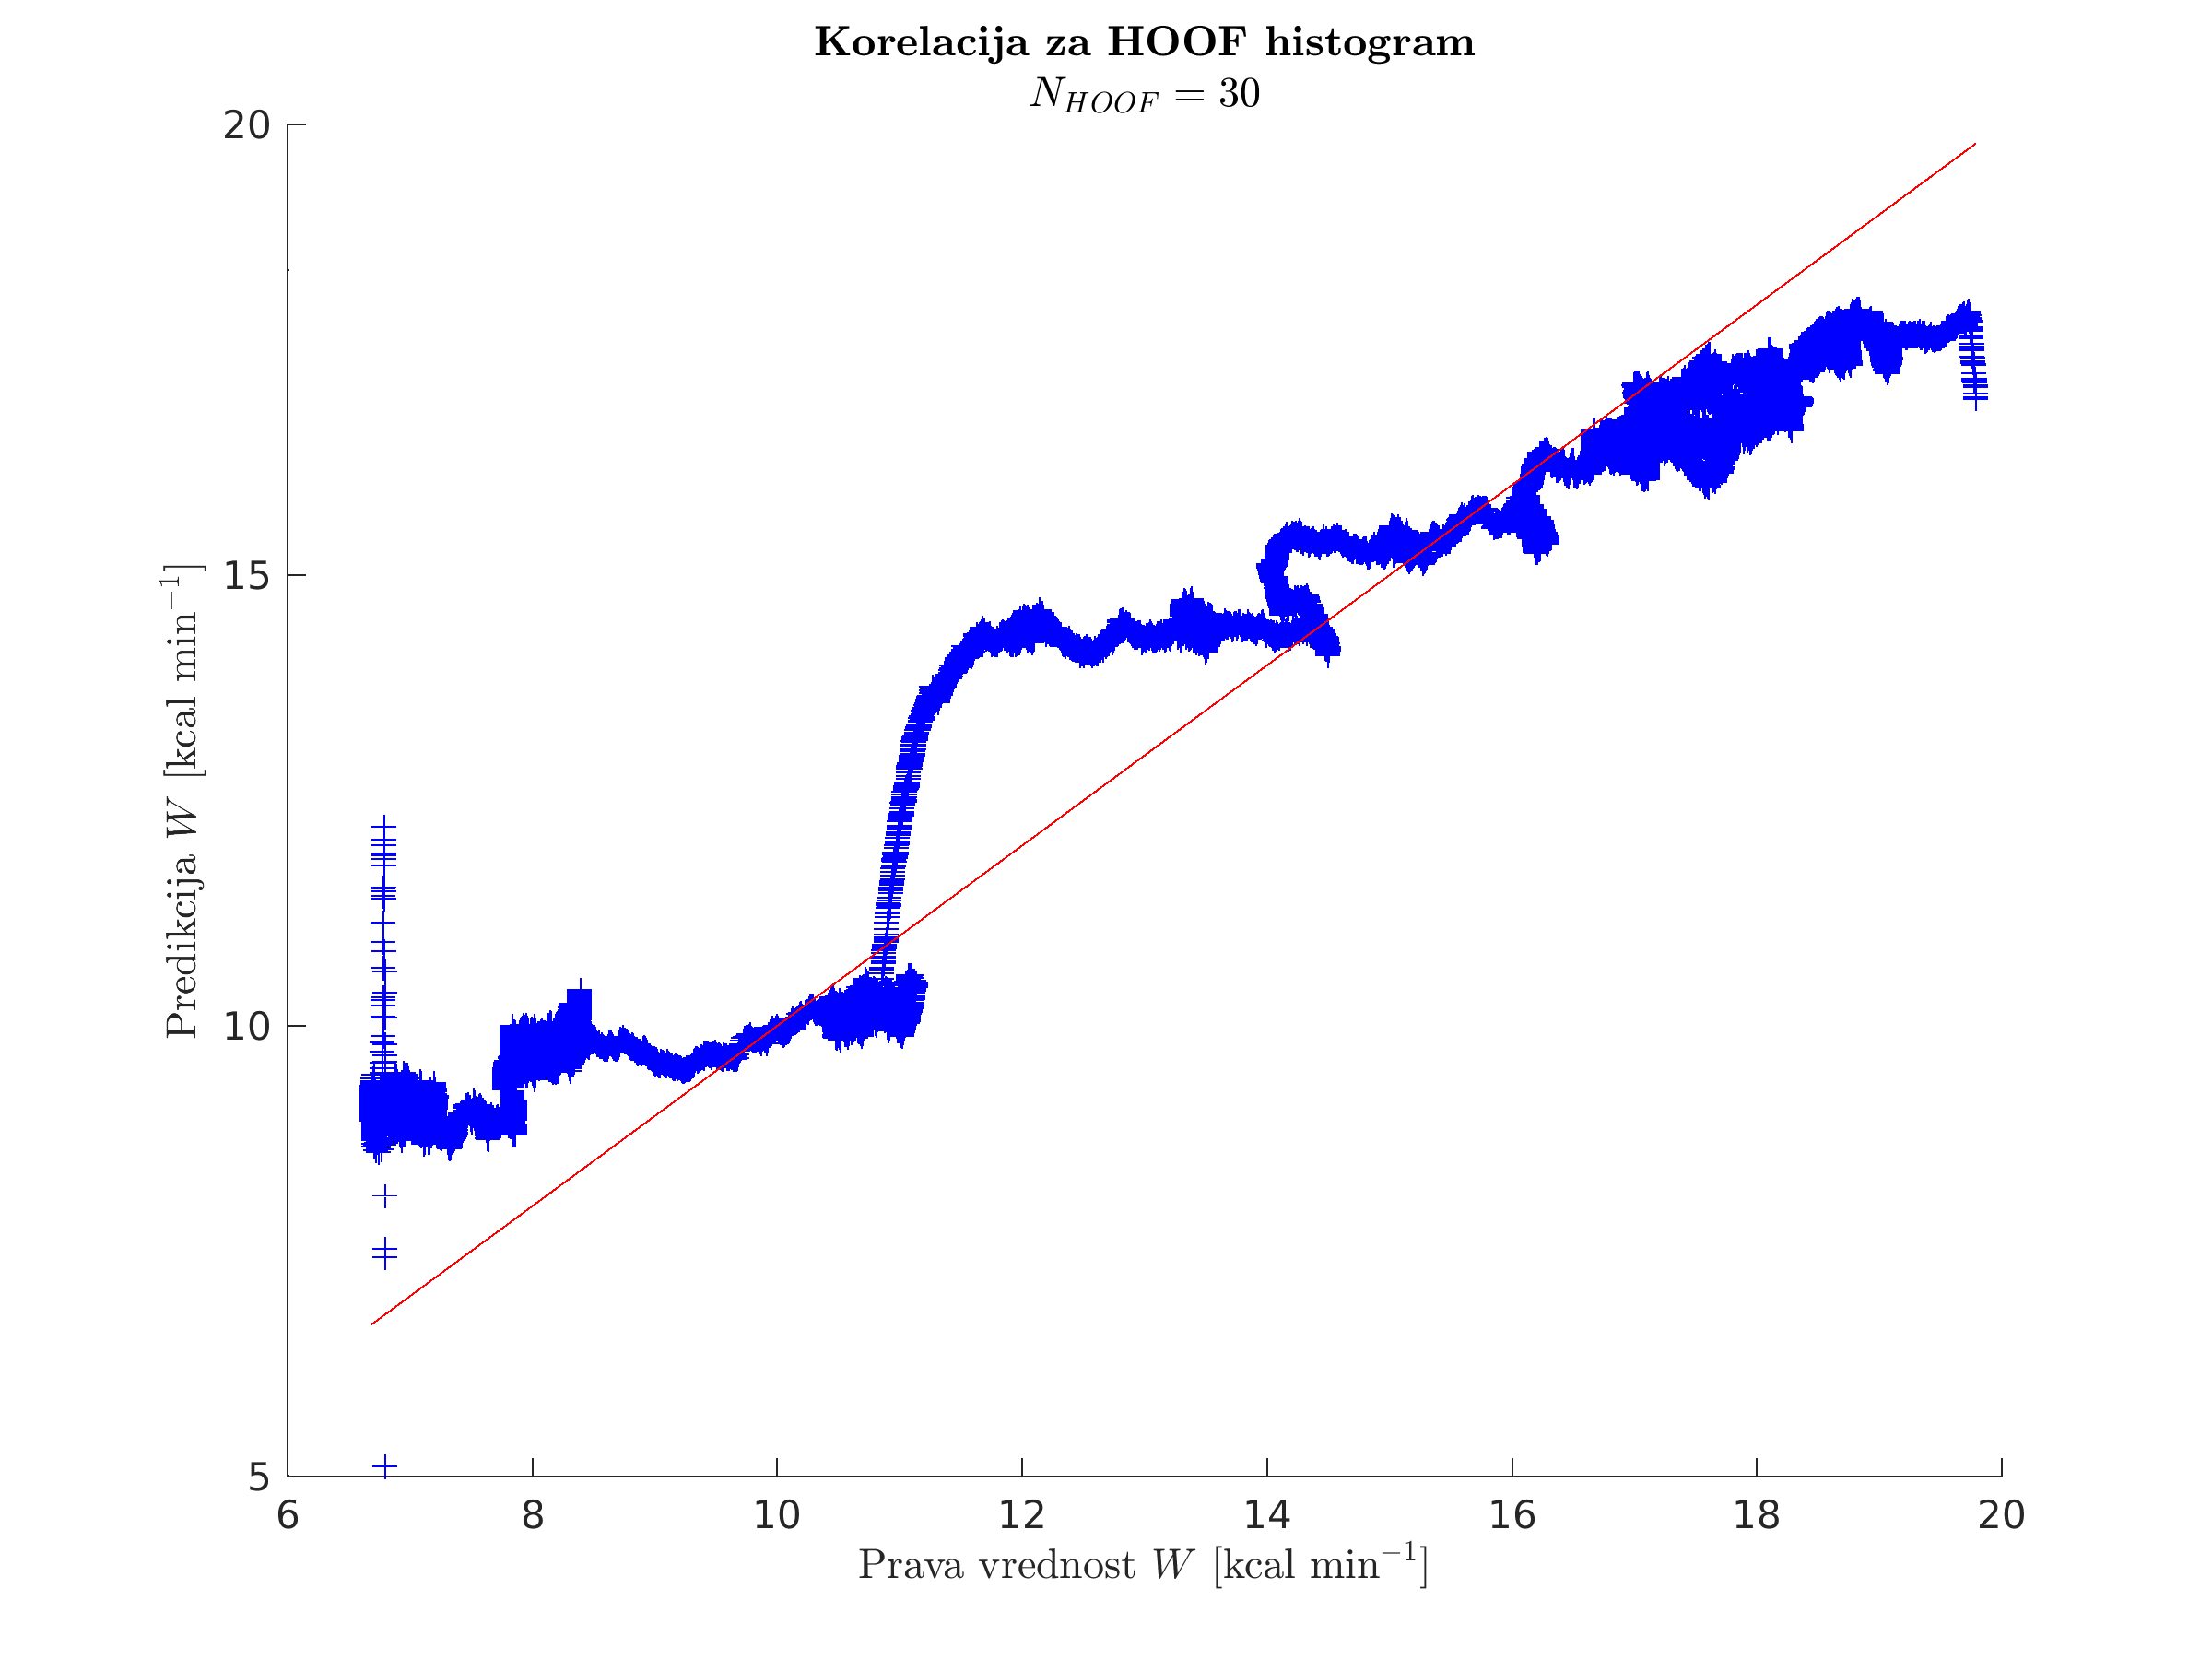
\includegraphics[width=\columnwidth]{./Slike/corr-hoof-30.png}
		\caption{Korelacija $N_{HOOF}=30$.}
		\label{fig:corr-hoof-30}
	\end{subfigure}
	~
	\begin{subfigure}[t]{0.45\columnwidth}
		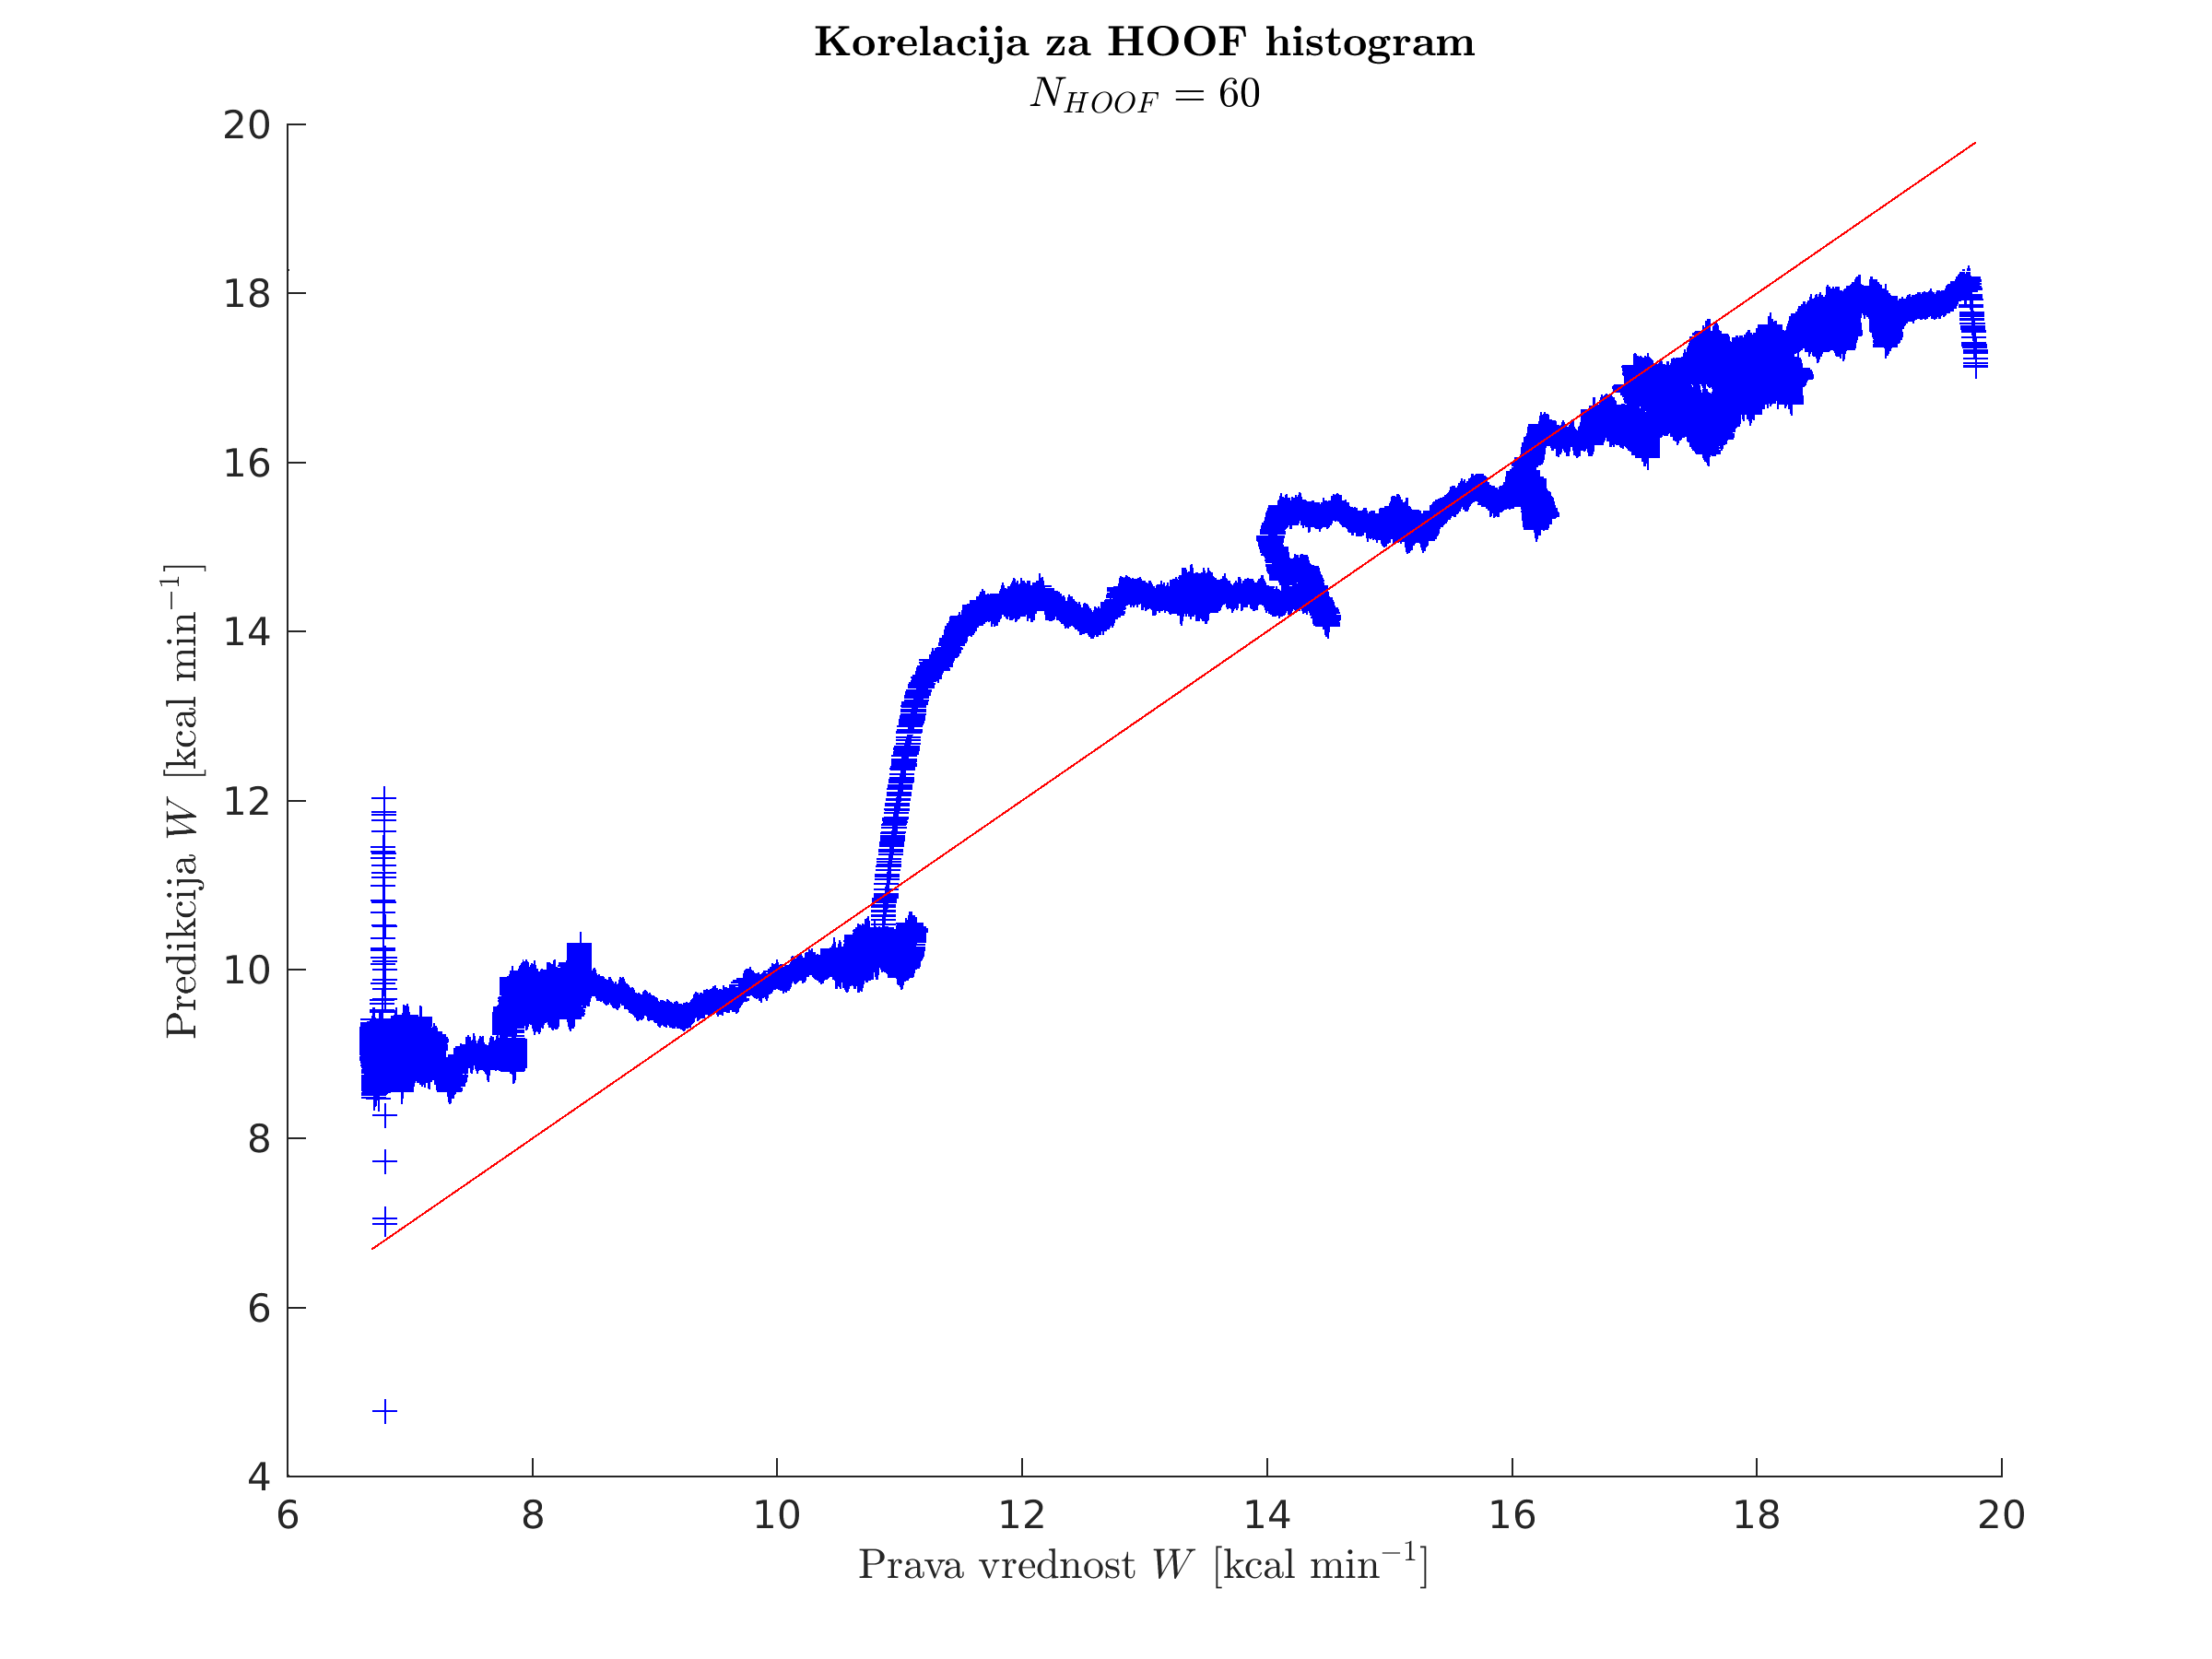
\includegraphics[width=\columnwidth]{./Slike/corr-hoof-60.png}
		\caption{Korelacija $N_{HOOF}=60$.}
		\label{fig:corr-hoof-60}
	\end{subfigure}
	~
	\begin{subfigure}[b]{0.45\columnwidth}
		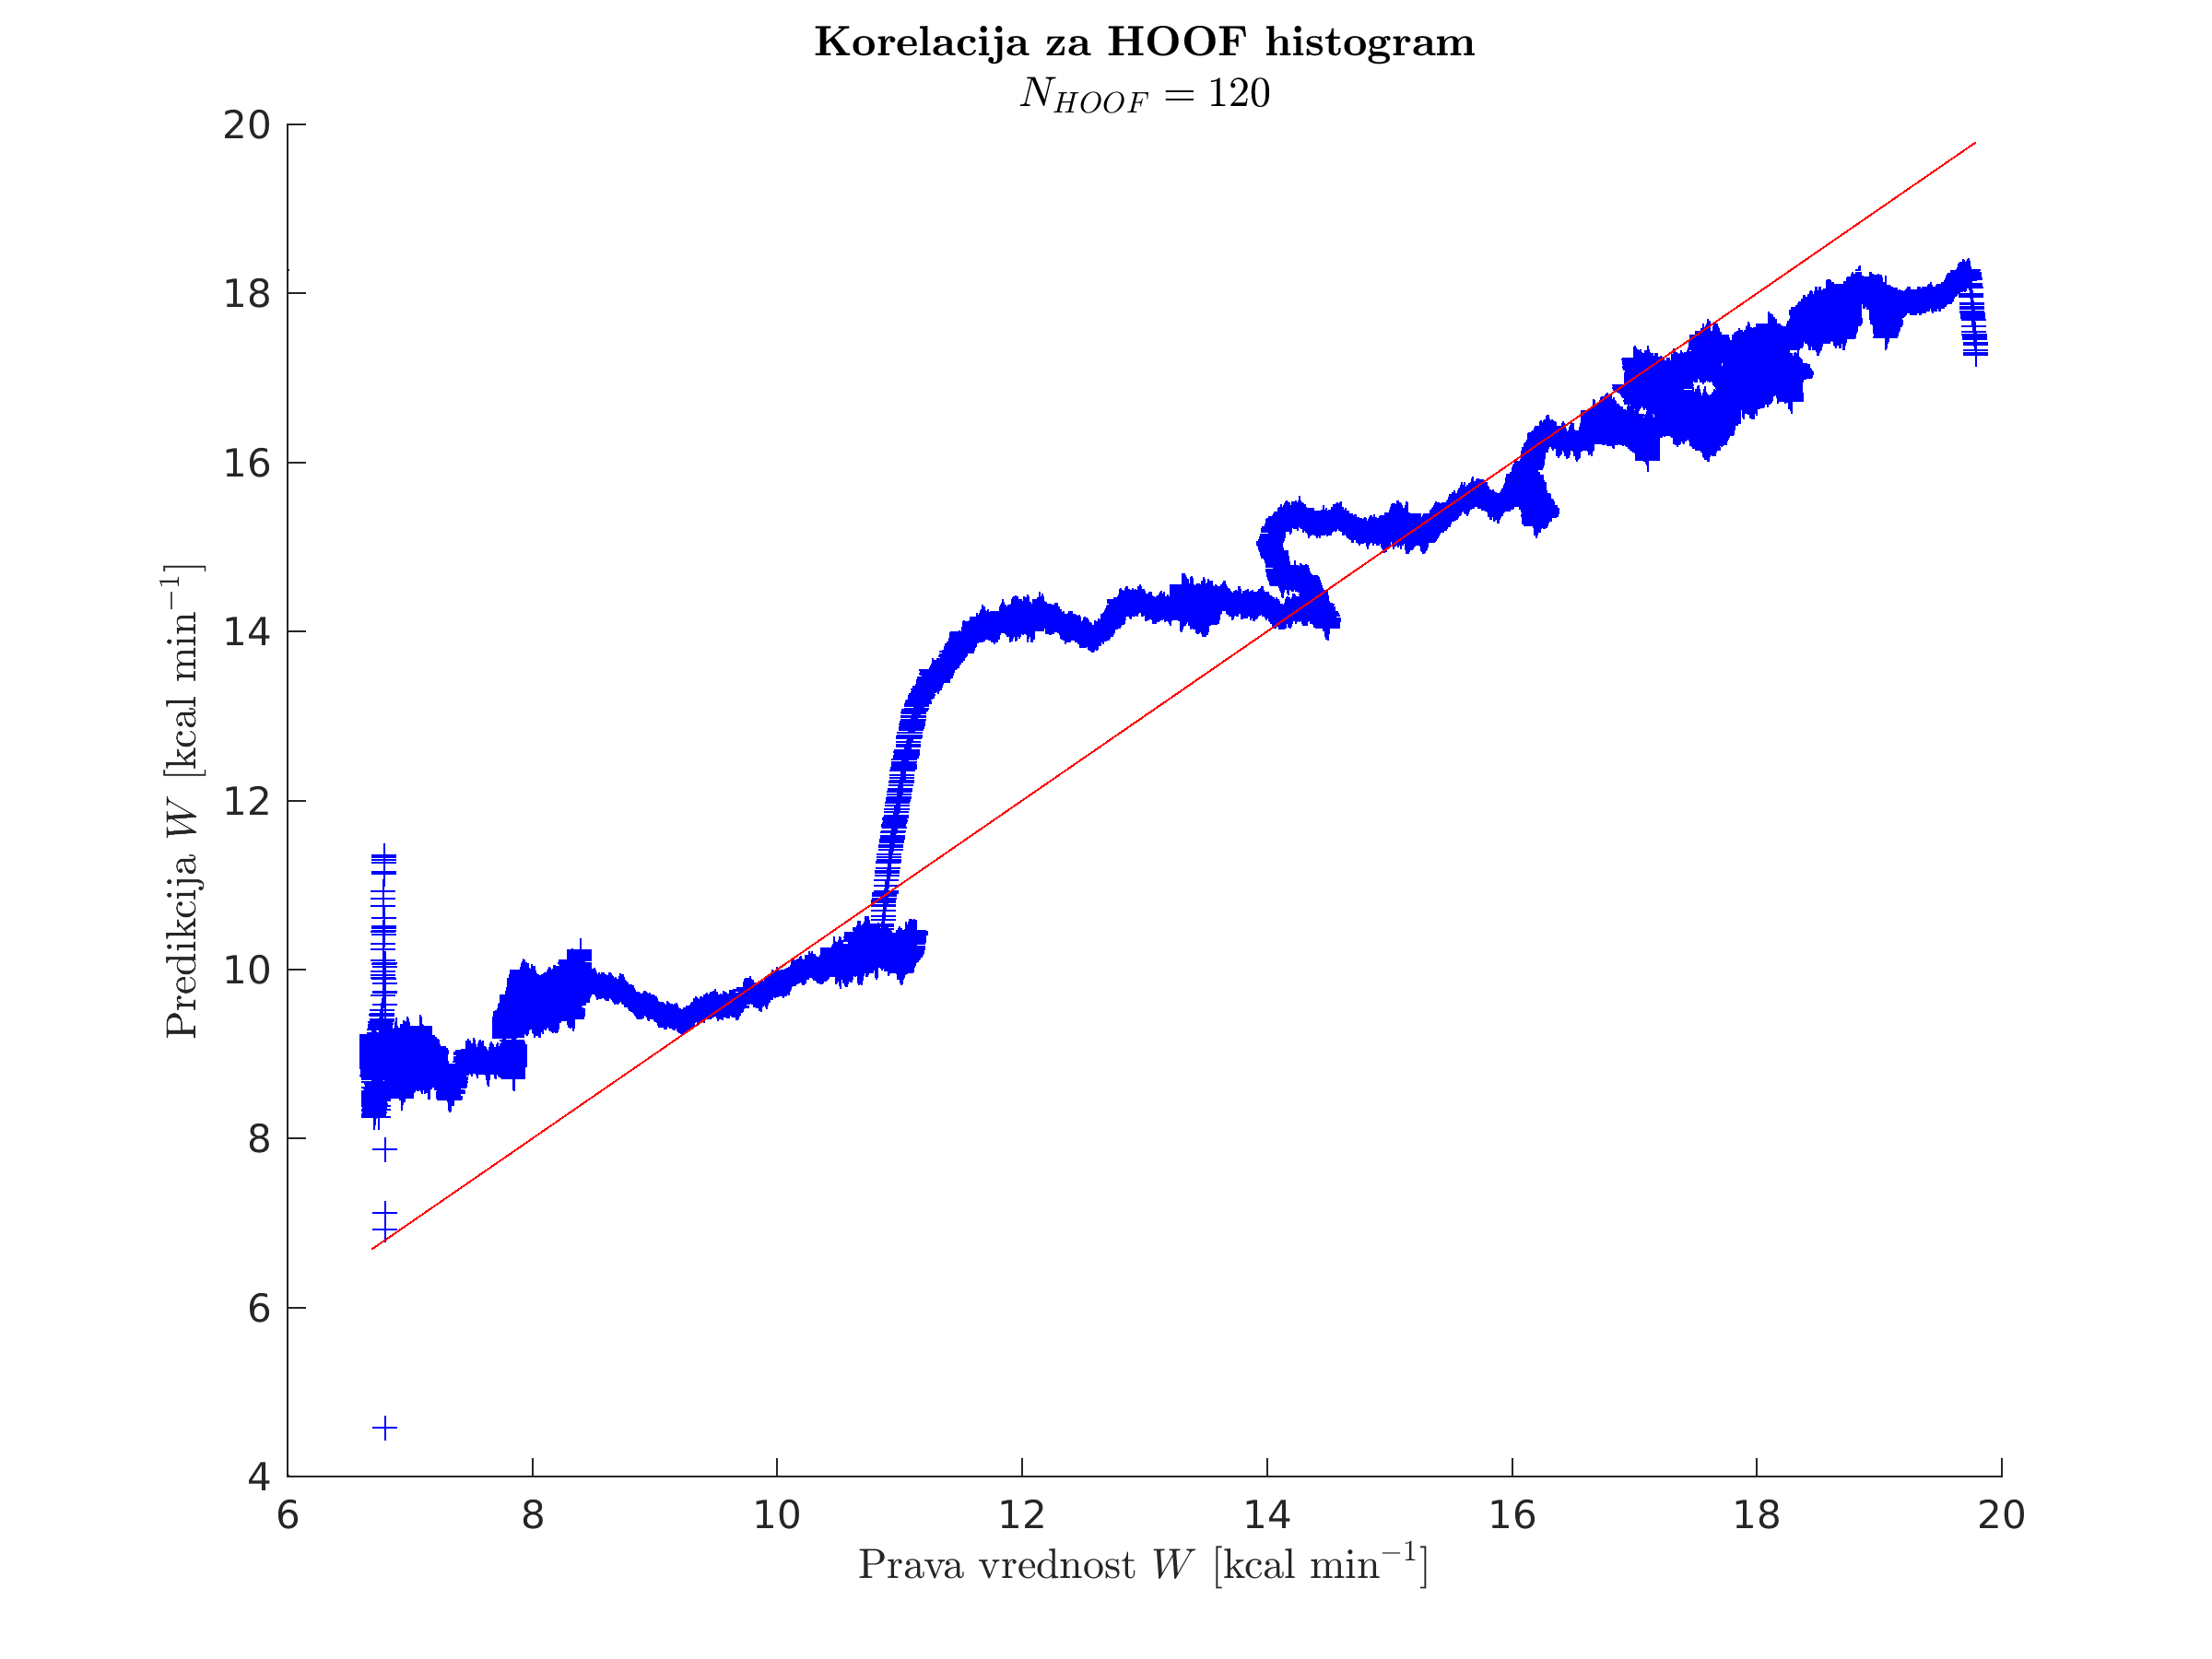
\includegraphics[width=\columnwidth]{./Slike/corr-hoof-120.png}
		\caption{Korelacija $N_{HOOF}=120$.}
		\label{fig:corr-hoof-120}
	\end{subfigure}
	~
	\begin{subfigure}[b]{0.45\columnwidth}
		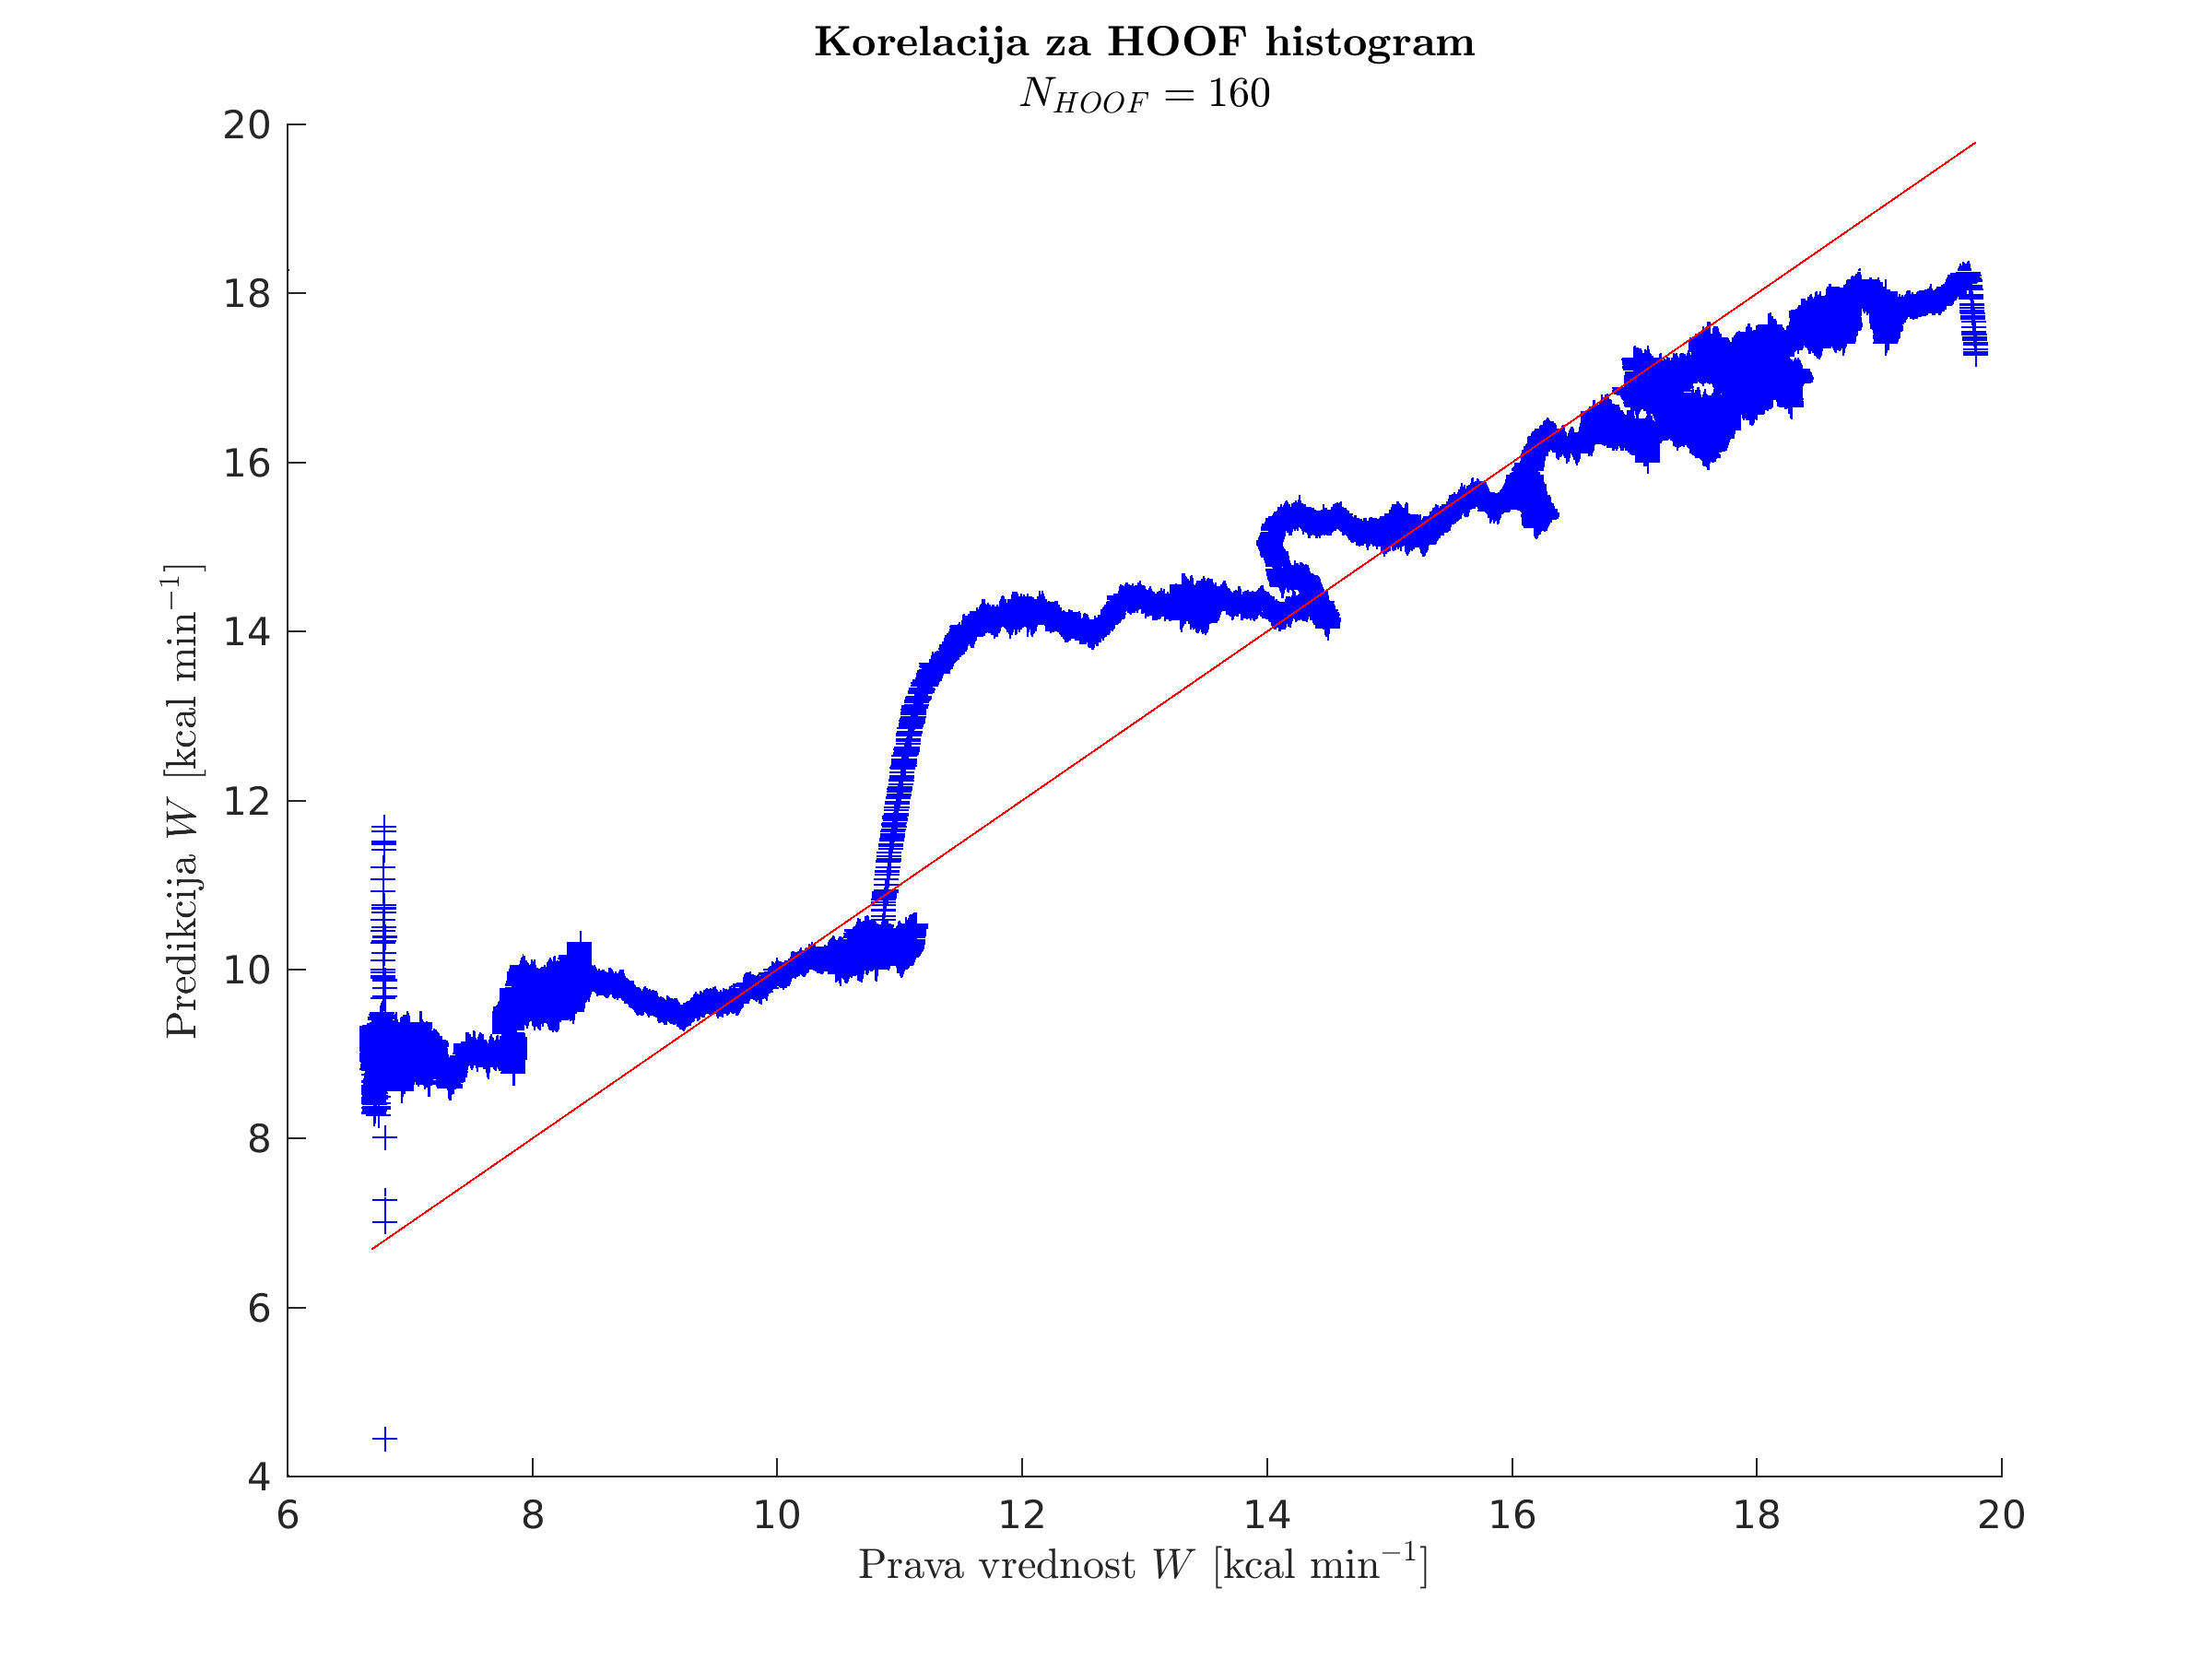
\includegraphics[width=\columnwidth]{./Slike/corr-hoof-160.png}
		\caption{Korelacija $N_{HOOF}=160$.}
		\label{fig:corr-hoof-160}
	\end{subfigure}
	\caption[Grafi korelacij modelov z različnim $N_{HOOF}$]{Grafi korelacij modelov z različnim številom stolpcev $N_{HOOF}$ HOOF deskriptorja. Rezultati so si zelo podobni.}
	\label{fig:corr-hoof}
\end{figure}












\subsubsection{Optimizacija HAFA deskriptorjev}\label{sec:rezultati-optimizacija-hafa}
Parameter $N_{HAFA}$ smo določili na podlagi rezultatov evaluacije v tabeli \ref{tab:nhafa} in grafov korelacije med referenčnimi podatki in predikcijo \ref{fig:corr-hafa}.

V tabeli \ref{tab:nhafa} lahko vidimo, da so rezultati praktično enaki. Za našo metodo smo izbrali $N_{HAFA}=60$, kar v grobem predstavlja $60$ različnih hitrosti z maksimalno amplitudo \SI{60}{px.f^{-1}}.

\begin{table}[htb]
	\centering
	\begin{tabular}{S[table-format=2.0] S[table-format=1.3] S[table-format=1.3] S[table-format=1.3] S[table-format=2.2]}
		\toprule
		\thead{$\mathbf{N_{HAFA}}$} & \thead{$\mathbf{r}$} & \thead{RAE} & \thead{RRSE} & \thead{nSV [\%]}\\
		\midrule%nSV
		30 & 0.984 & 0.213 & 0.231 & 62.08 \\%17879/28799
		\boldentry{2.0}{60} & \boldentry{1.3}{0.984} & \boldentry{1.3}{0.211} & \boldentry{1.3}{0.228} & \boldentry{2.2}{62.60} \\%18028
		120 & 0.984 & 0.211 & 0.228 & 62.63 \\%18037
		160 & 0.984 & 0.211 & 0.228 & 62.63 \\%18037
		\bottomrule
	\end{tabular}
	\caption[Rezultati evaluacije modelov z različnim $N_{HAFA}$]{Rezultati evaluacije modelov z različnim številom stolpcev $N_{HAFA}$ HAFA deskriptorja. Optimalni rezultati so odebeljeni.}
	\label{tab:nhafa}
\end{table}

\begin{figure}[htb]
	\centering
	\begin{subfigure}[t]{0.45\columnwidth}
		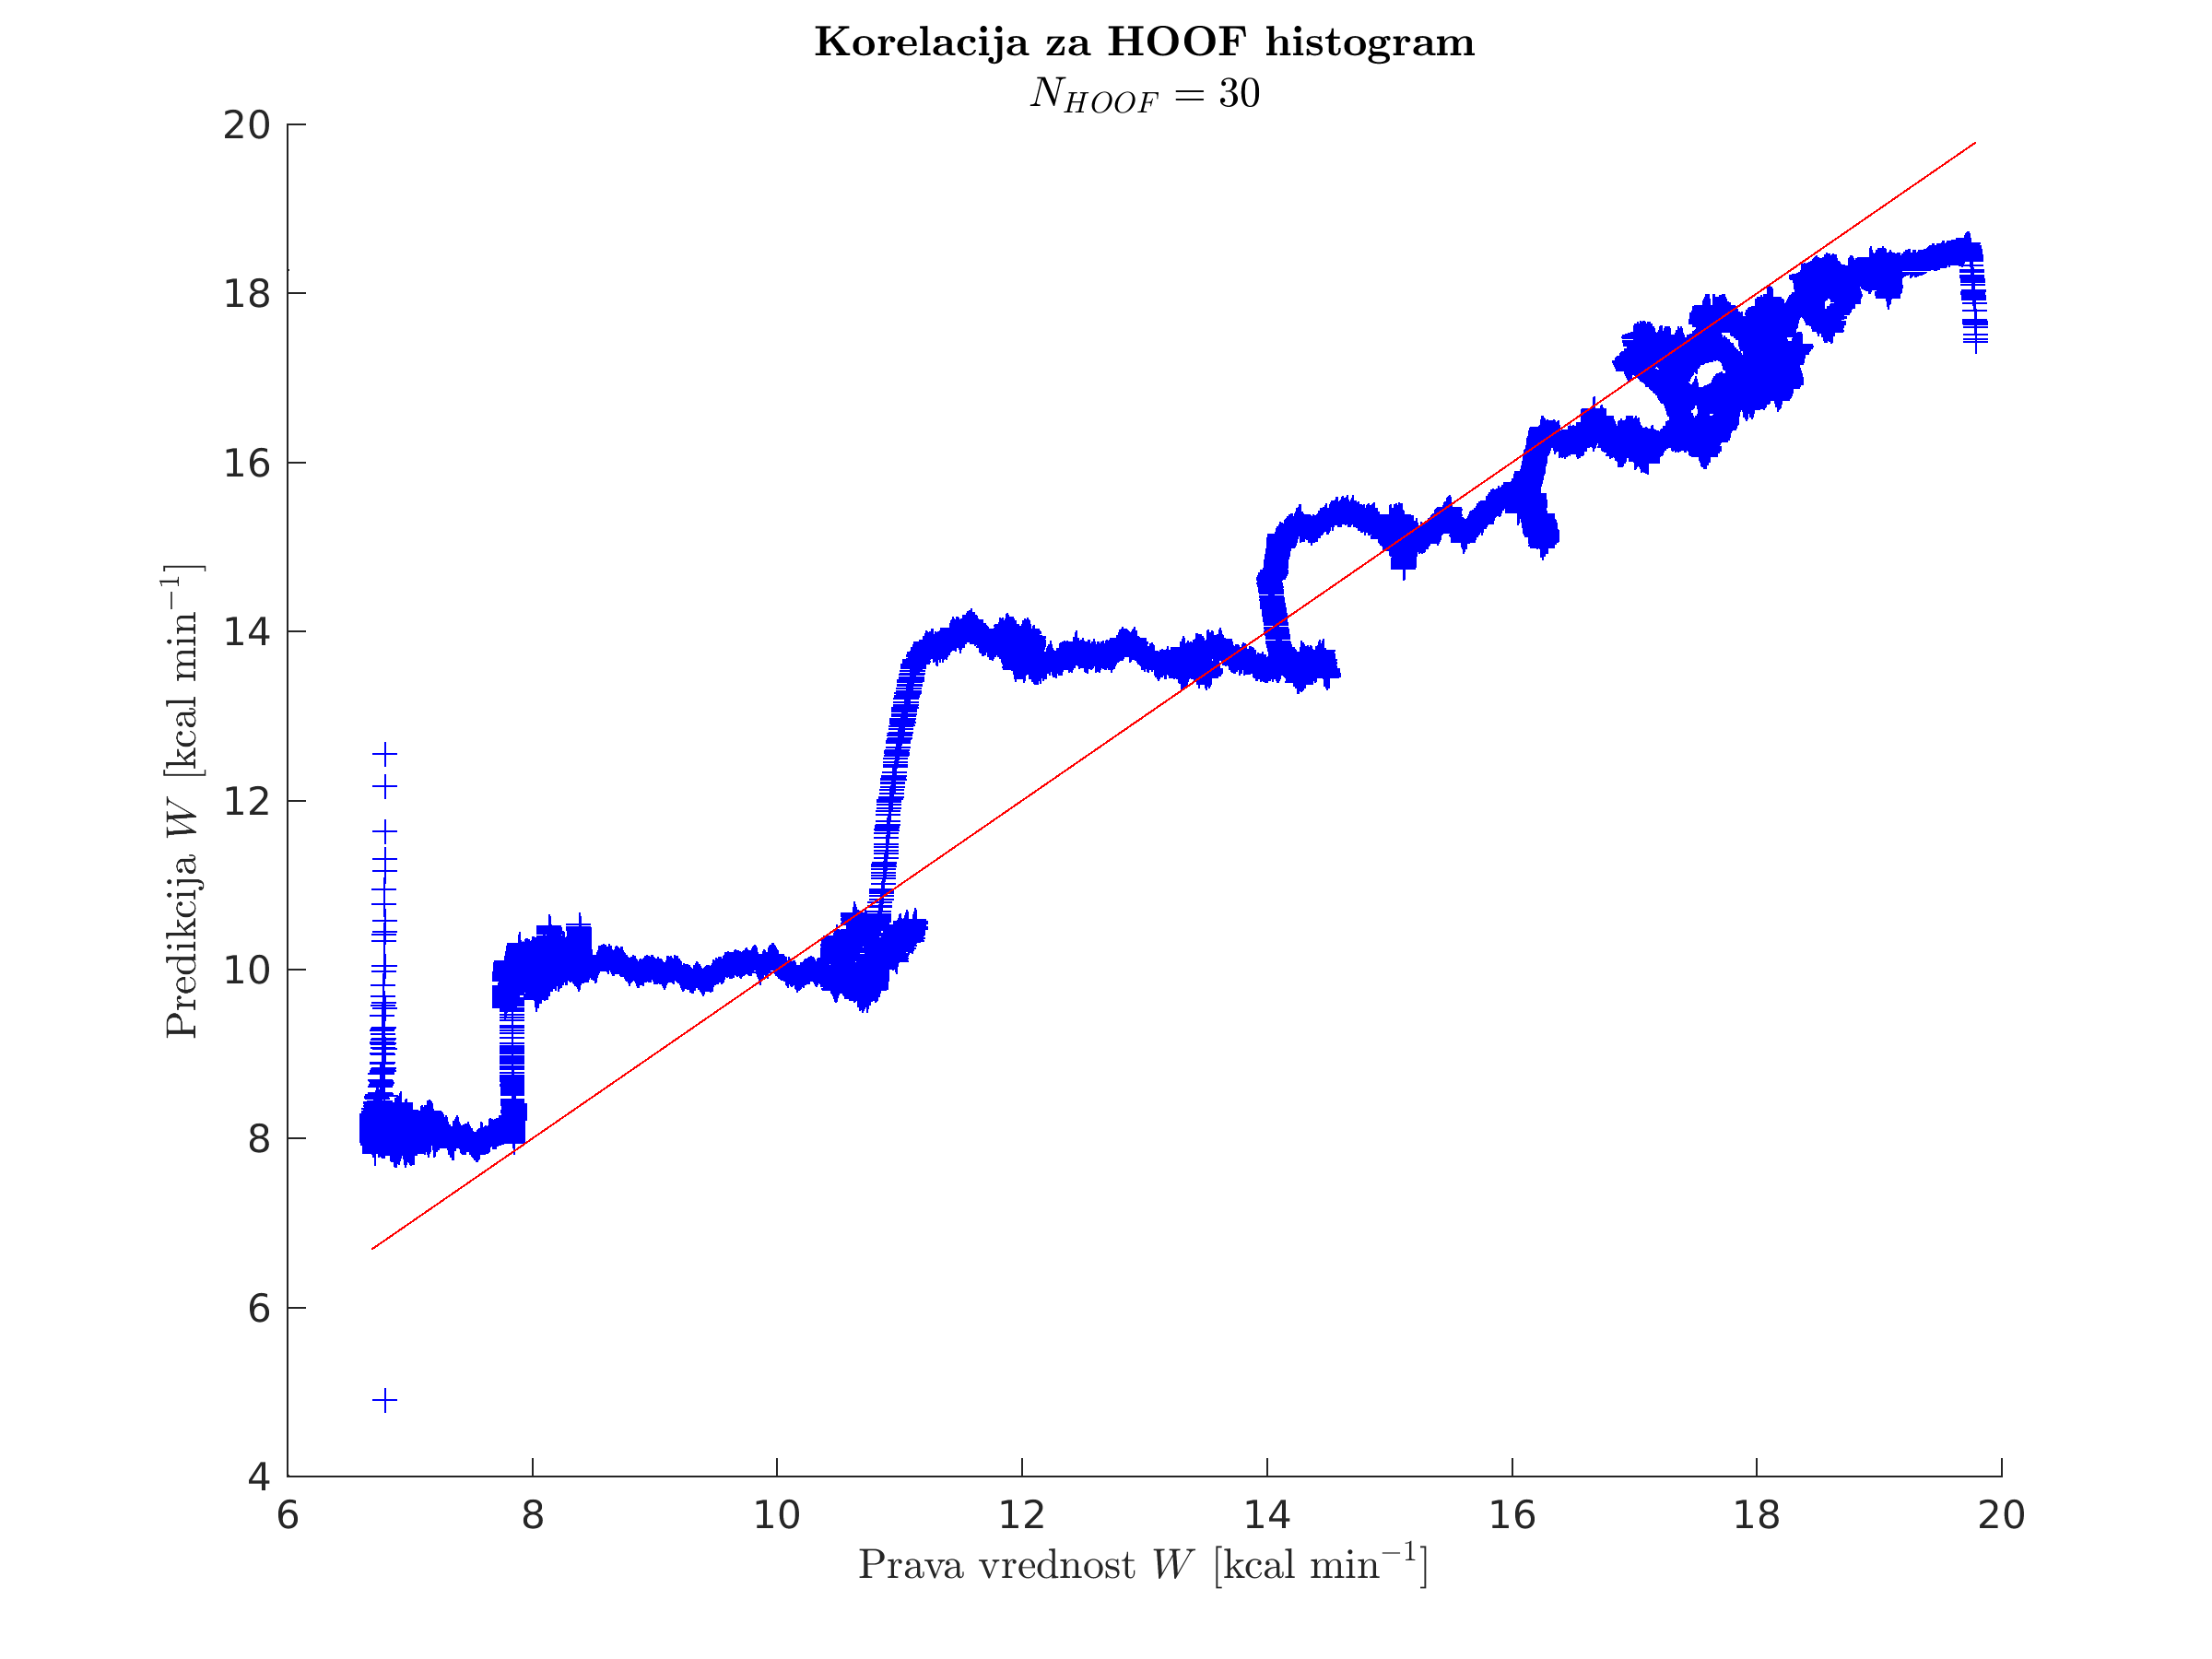
\includegraphics[width=\columnwidth]{./Slike/corr-hafa-30.png}
		\caption{Korelacija $N_{HAFA}=30$.}
		\label{fig:corr-hafa-30}
	\end{subfigure}
	~
	\begin{subfigure}[t]{0.45\columnwidth}
		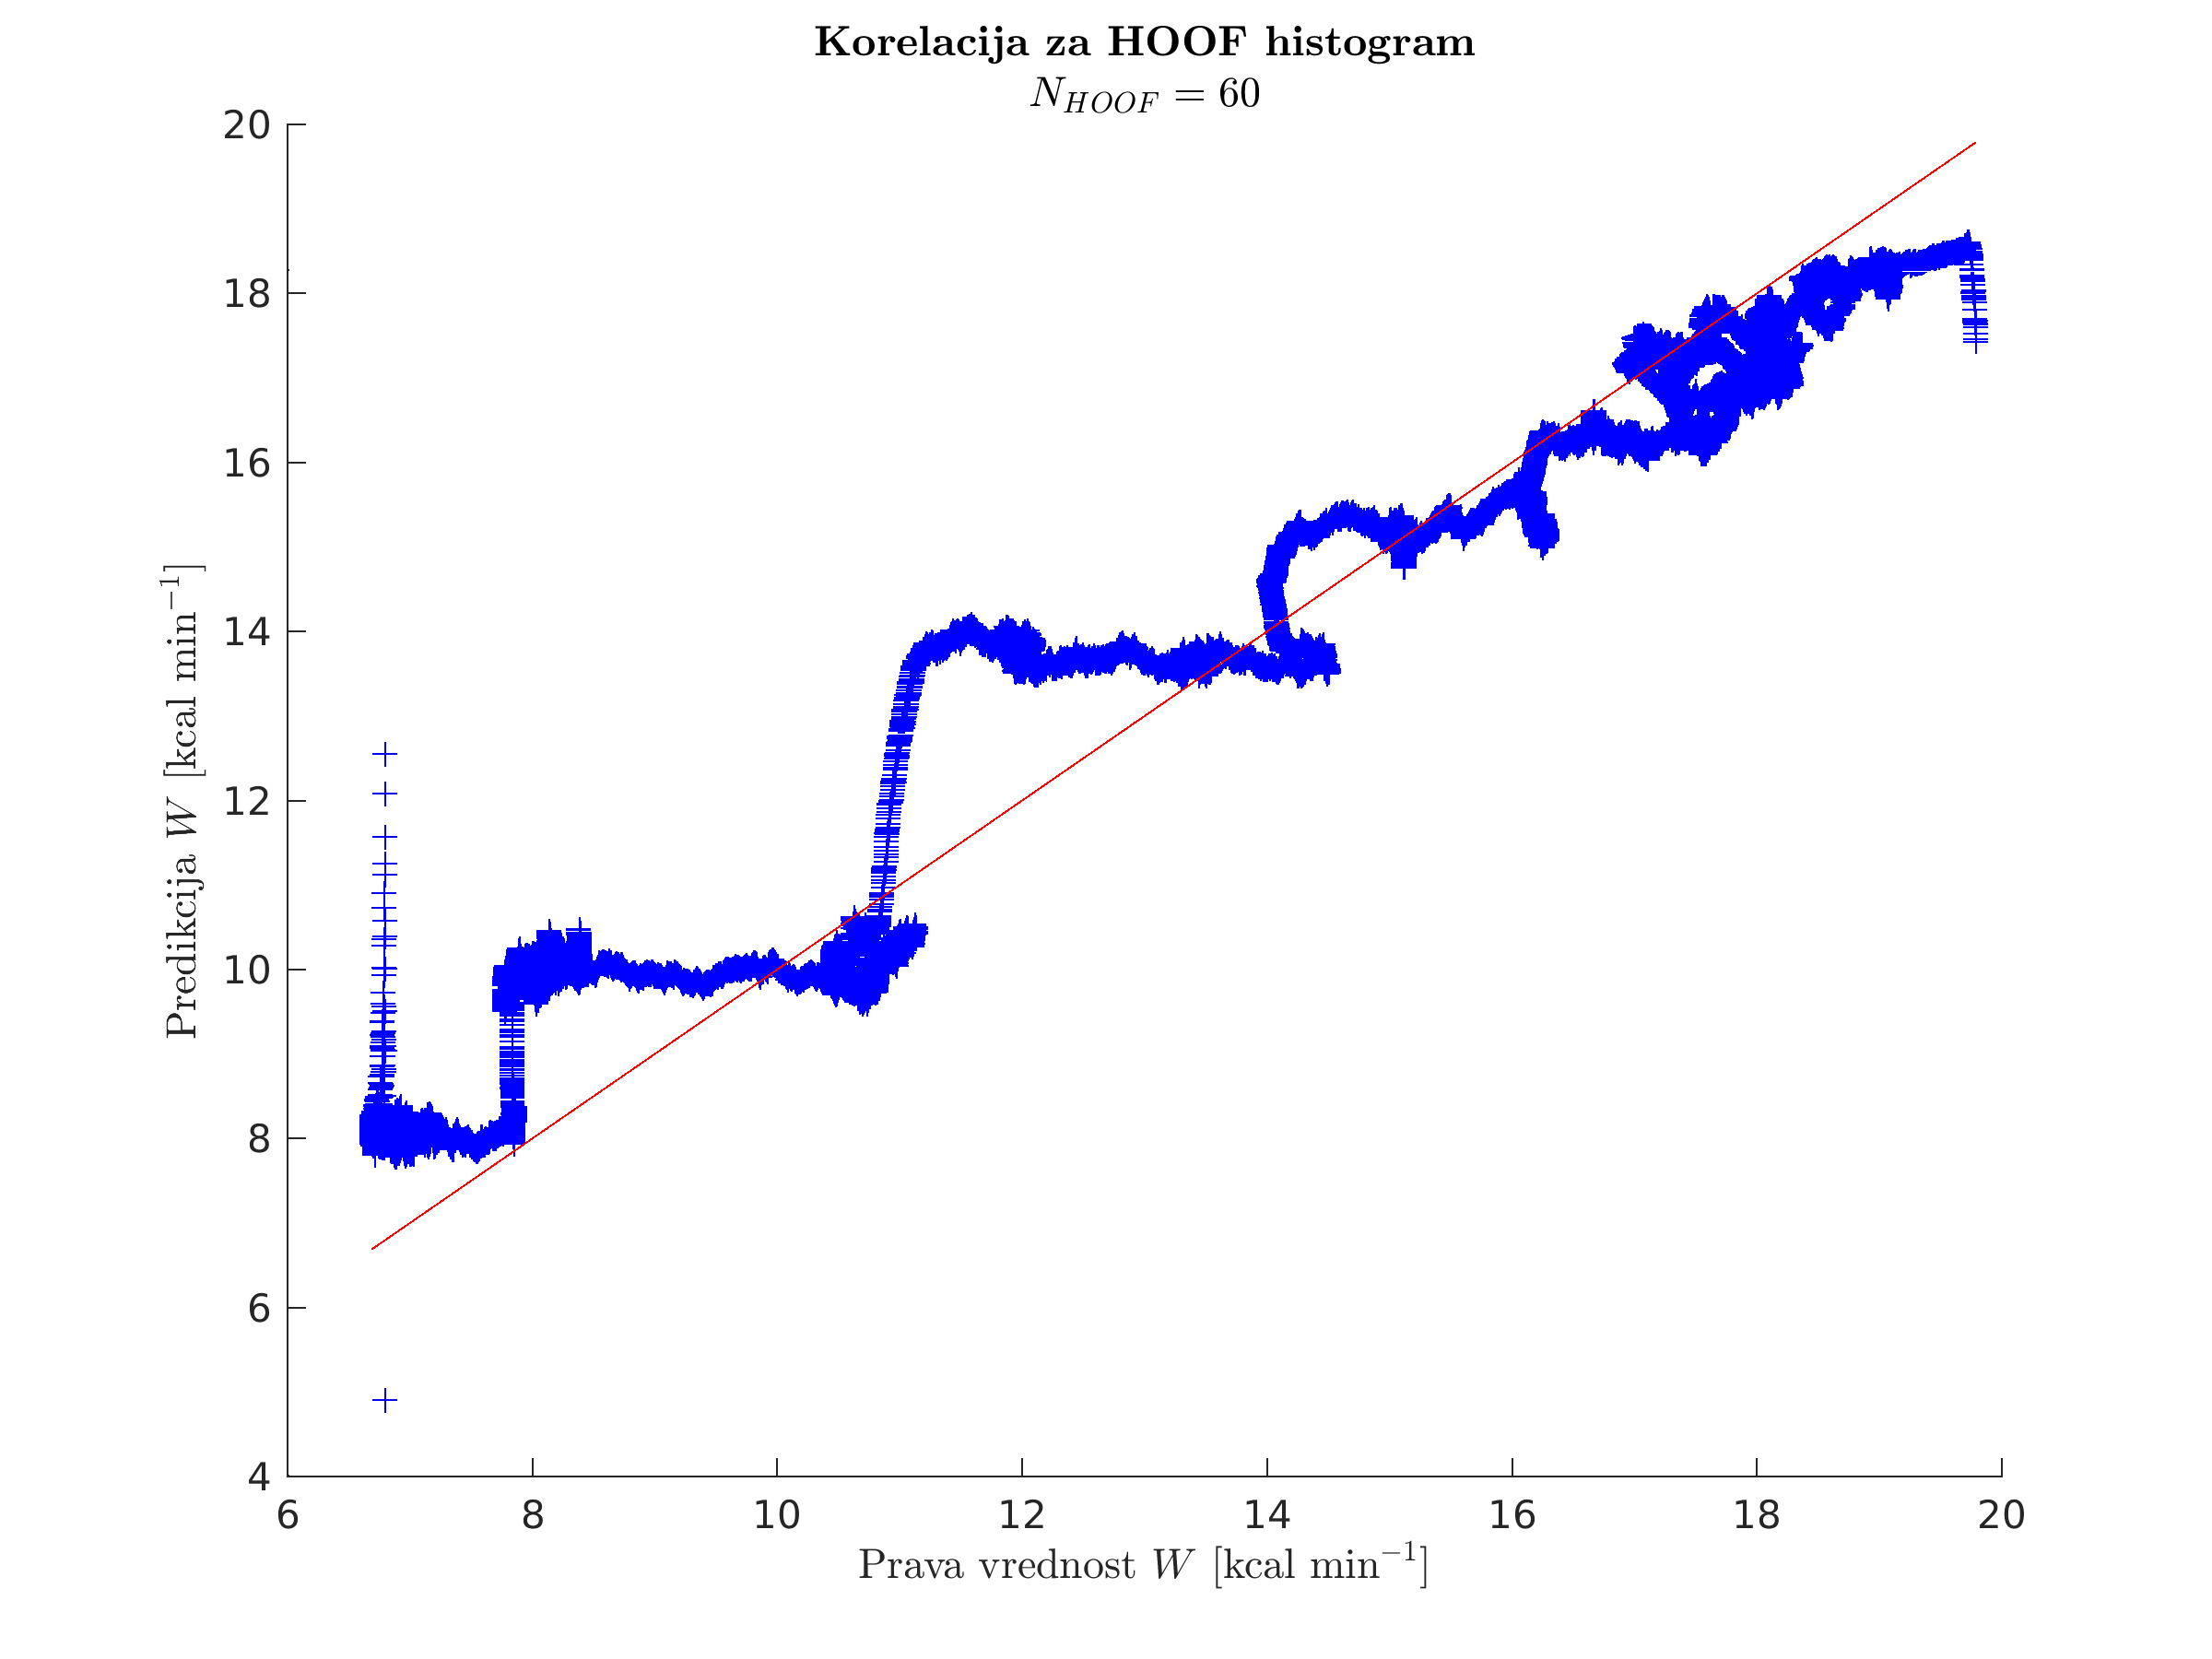
\includegraphics[width=\columnwidth]{./Slike/corr-hafa-60.png}
		\caption{Korelacija $N_{HAFA}=60$.}
		\label{fig:corr-hafa-60}
	\end{subfigure}
	~
	\begin{subfigure}[b]{0.45\columnwidth}
		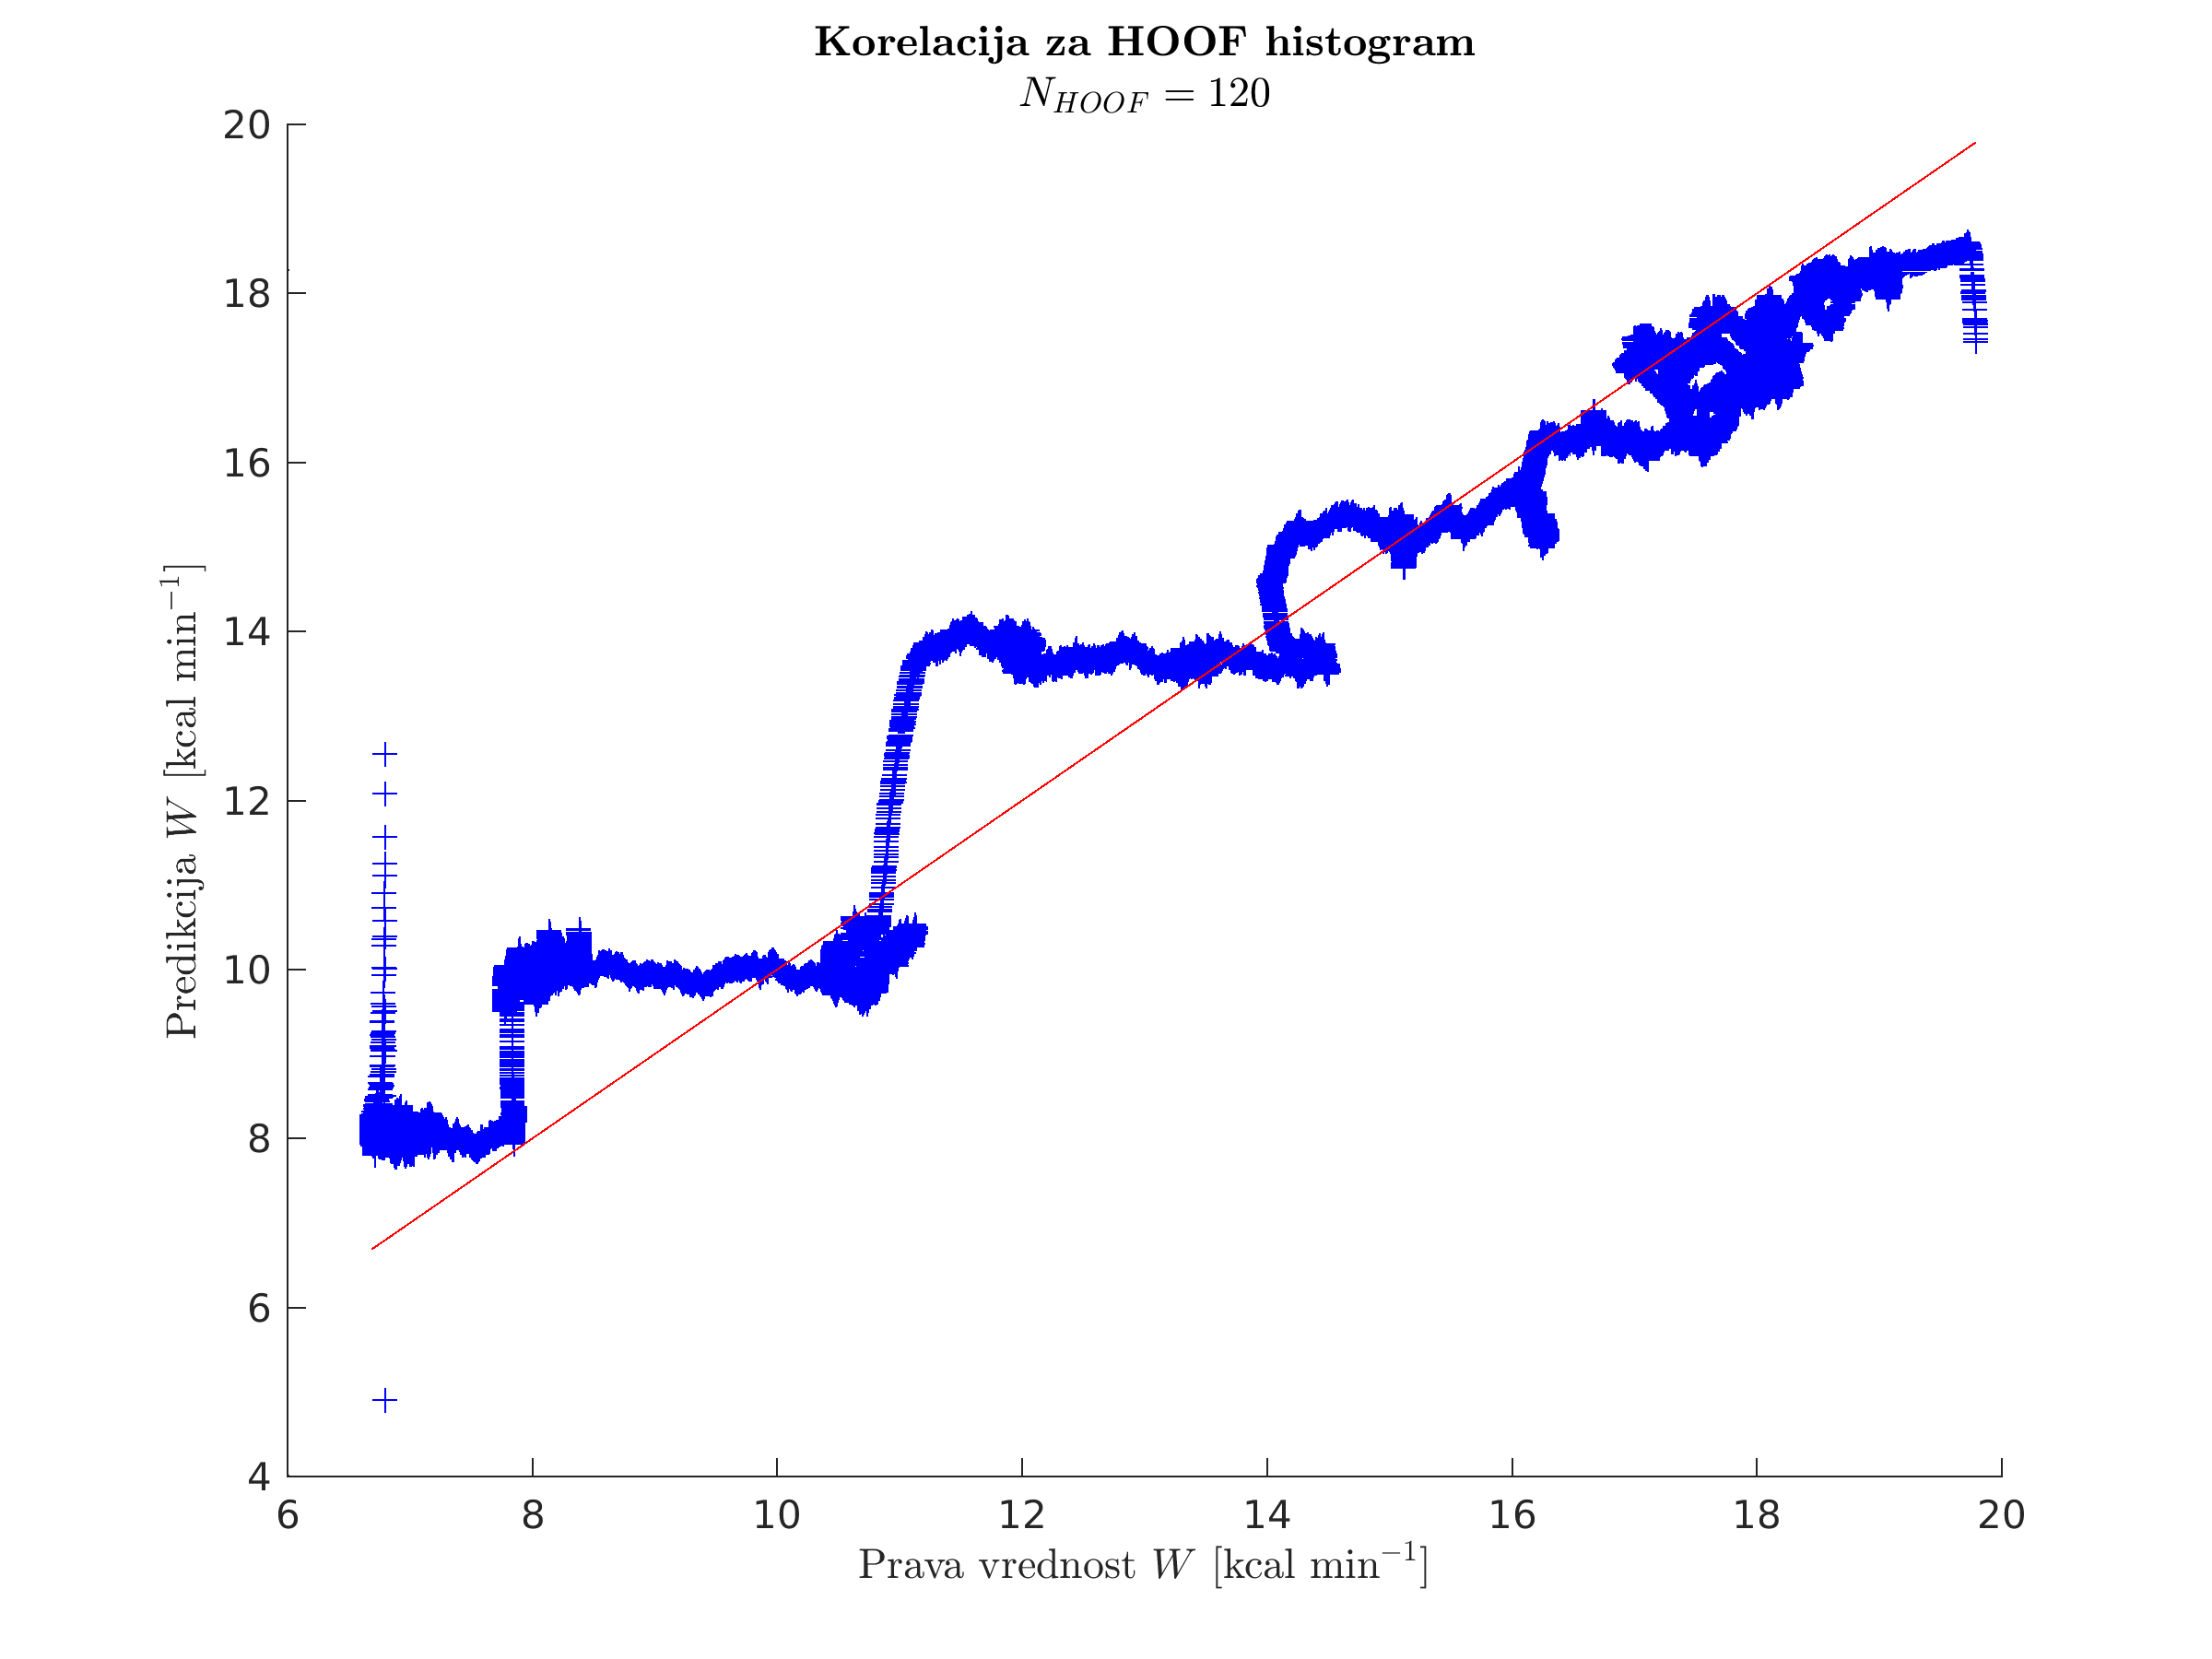
\includegraphics[width=\columnwidth]{./Slike/corr-hafa-120.png}
		\caption{Korelacija $N_{HAFA}=120$.}
		\label{fig:corr-hafa-120}
	\end{subfigure}
	~
	\begin{subfigure}[b]{0.45\columnwidth}
		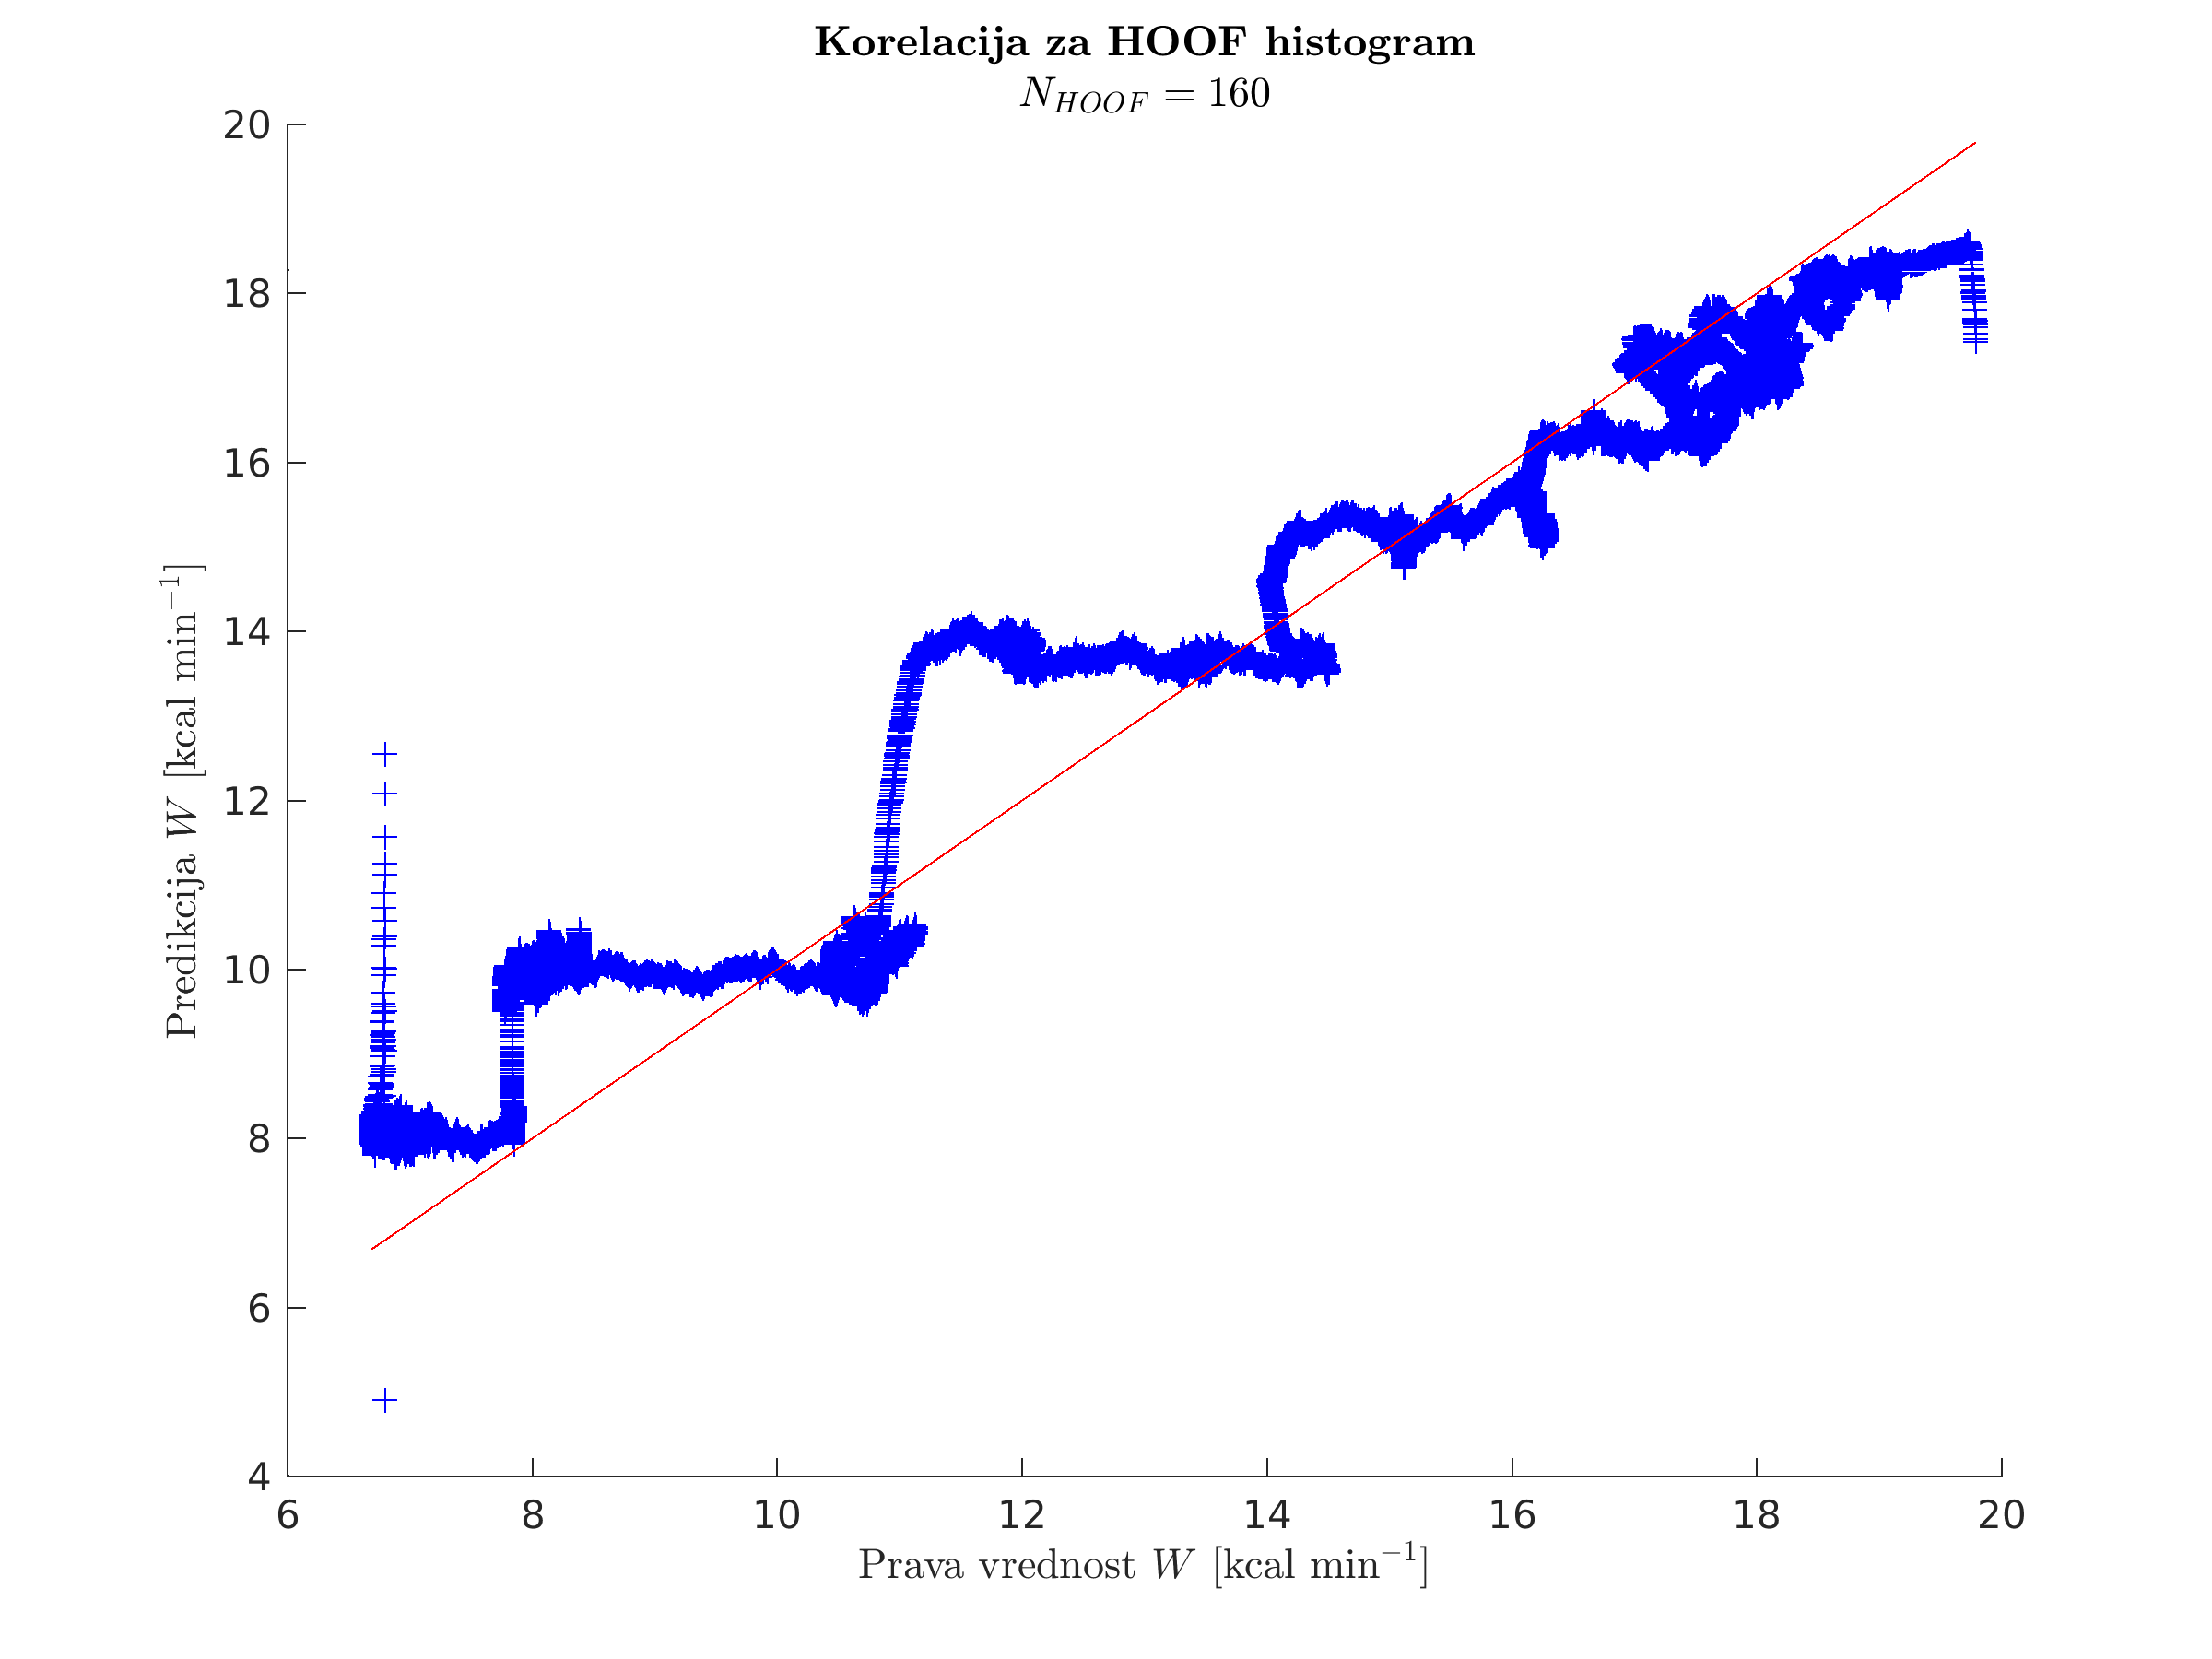
\includegraphics[width=\columnwidth]{./Slike/corr-hafa-160.png}
		\caption{Korelacija $N_{HAFA}=160$.}
		\label{fig:corr-hafa-160}
	\end{subfigure}
	\caption[Grafi korelacij modelov z različnim $N_{HAFA}$]{Grafi korelacij modelov z različnim številom stolpcev $N_{HAFA}$ HAFA deskriptorja. Rezultati so si zelo podobni.}
	\label{fig:corr-hafa}
\end{figure}







\subsubsection{Rarzširitev HOOF deskriptorja}\label{sec:rezultati-razsiritev-hoof}
\begin{table}[htb]
	\centering
	\begin{tabular}{l S[table-format=1.3] S[table-format=1.3] S[table-format=1.3] S[table-format=2.2]}
		\toprule
		\textbf{Deskriptor} & \thead{$\mathbf{r}$} & \thead{RAE} & \thead{RRSE} & \thead{nSV [\%]}\\
		\midrule%nSV
		HOOF & 0.992 & 0.336 & 0.317 & \boldentry{2.2}{82.34} \\%2187/2656
		\textbf{HOOF-HAFA} & \boldentry{1.3}{0.991} & \boldentry{1.3}{0.157} & \boldentry{1.3}{0.205} & 89.53 \\%2378
		\bottomrule
	\end{tabular}
	\caption[Rezultati evaluacije modelov z različnim deskriptorjem]{Rezultati evaluacije modelov z različnim deskriptorjem. Optimalni rezultati so odebeljeni. Vidimo lahko, da se bolje odnese razširjeni deskriptor HOOF-HAFA, čeprav model uporablja več podpornih vektorjev. }
	\label{tab:izbira}
\end{table}



\begin{figure}[!htb]
	\centering
	\begin{subfigure}[t]{0.45\columnwidth}
		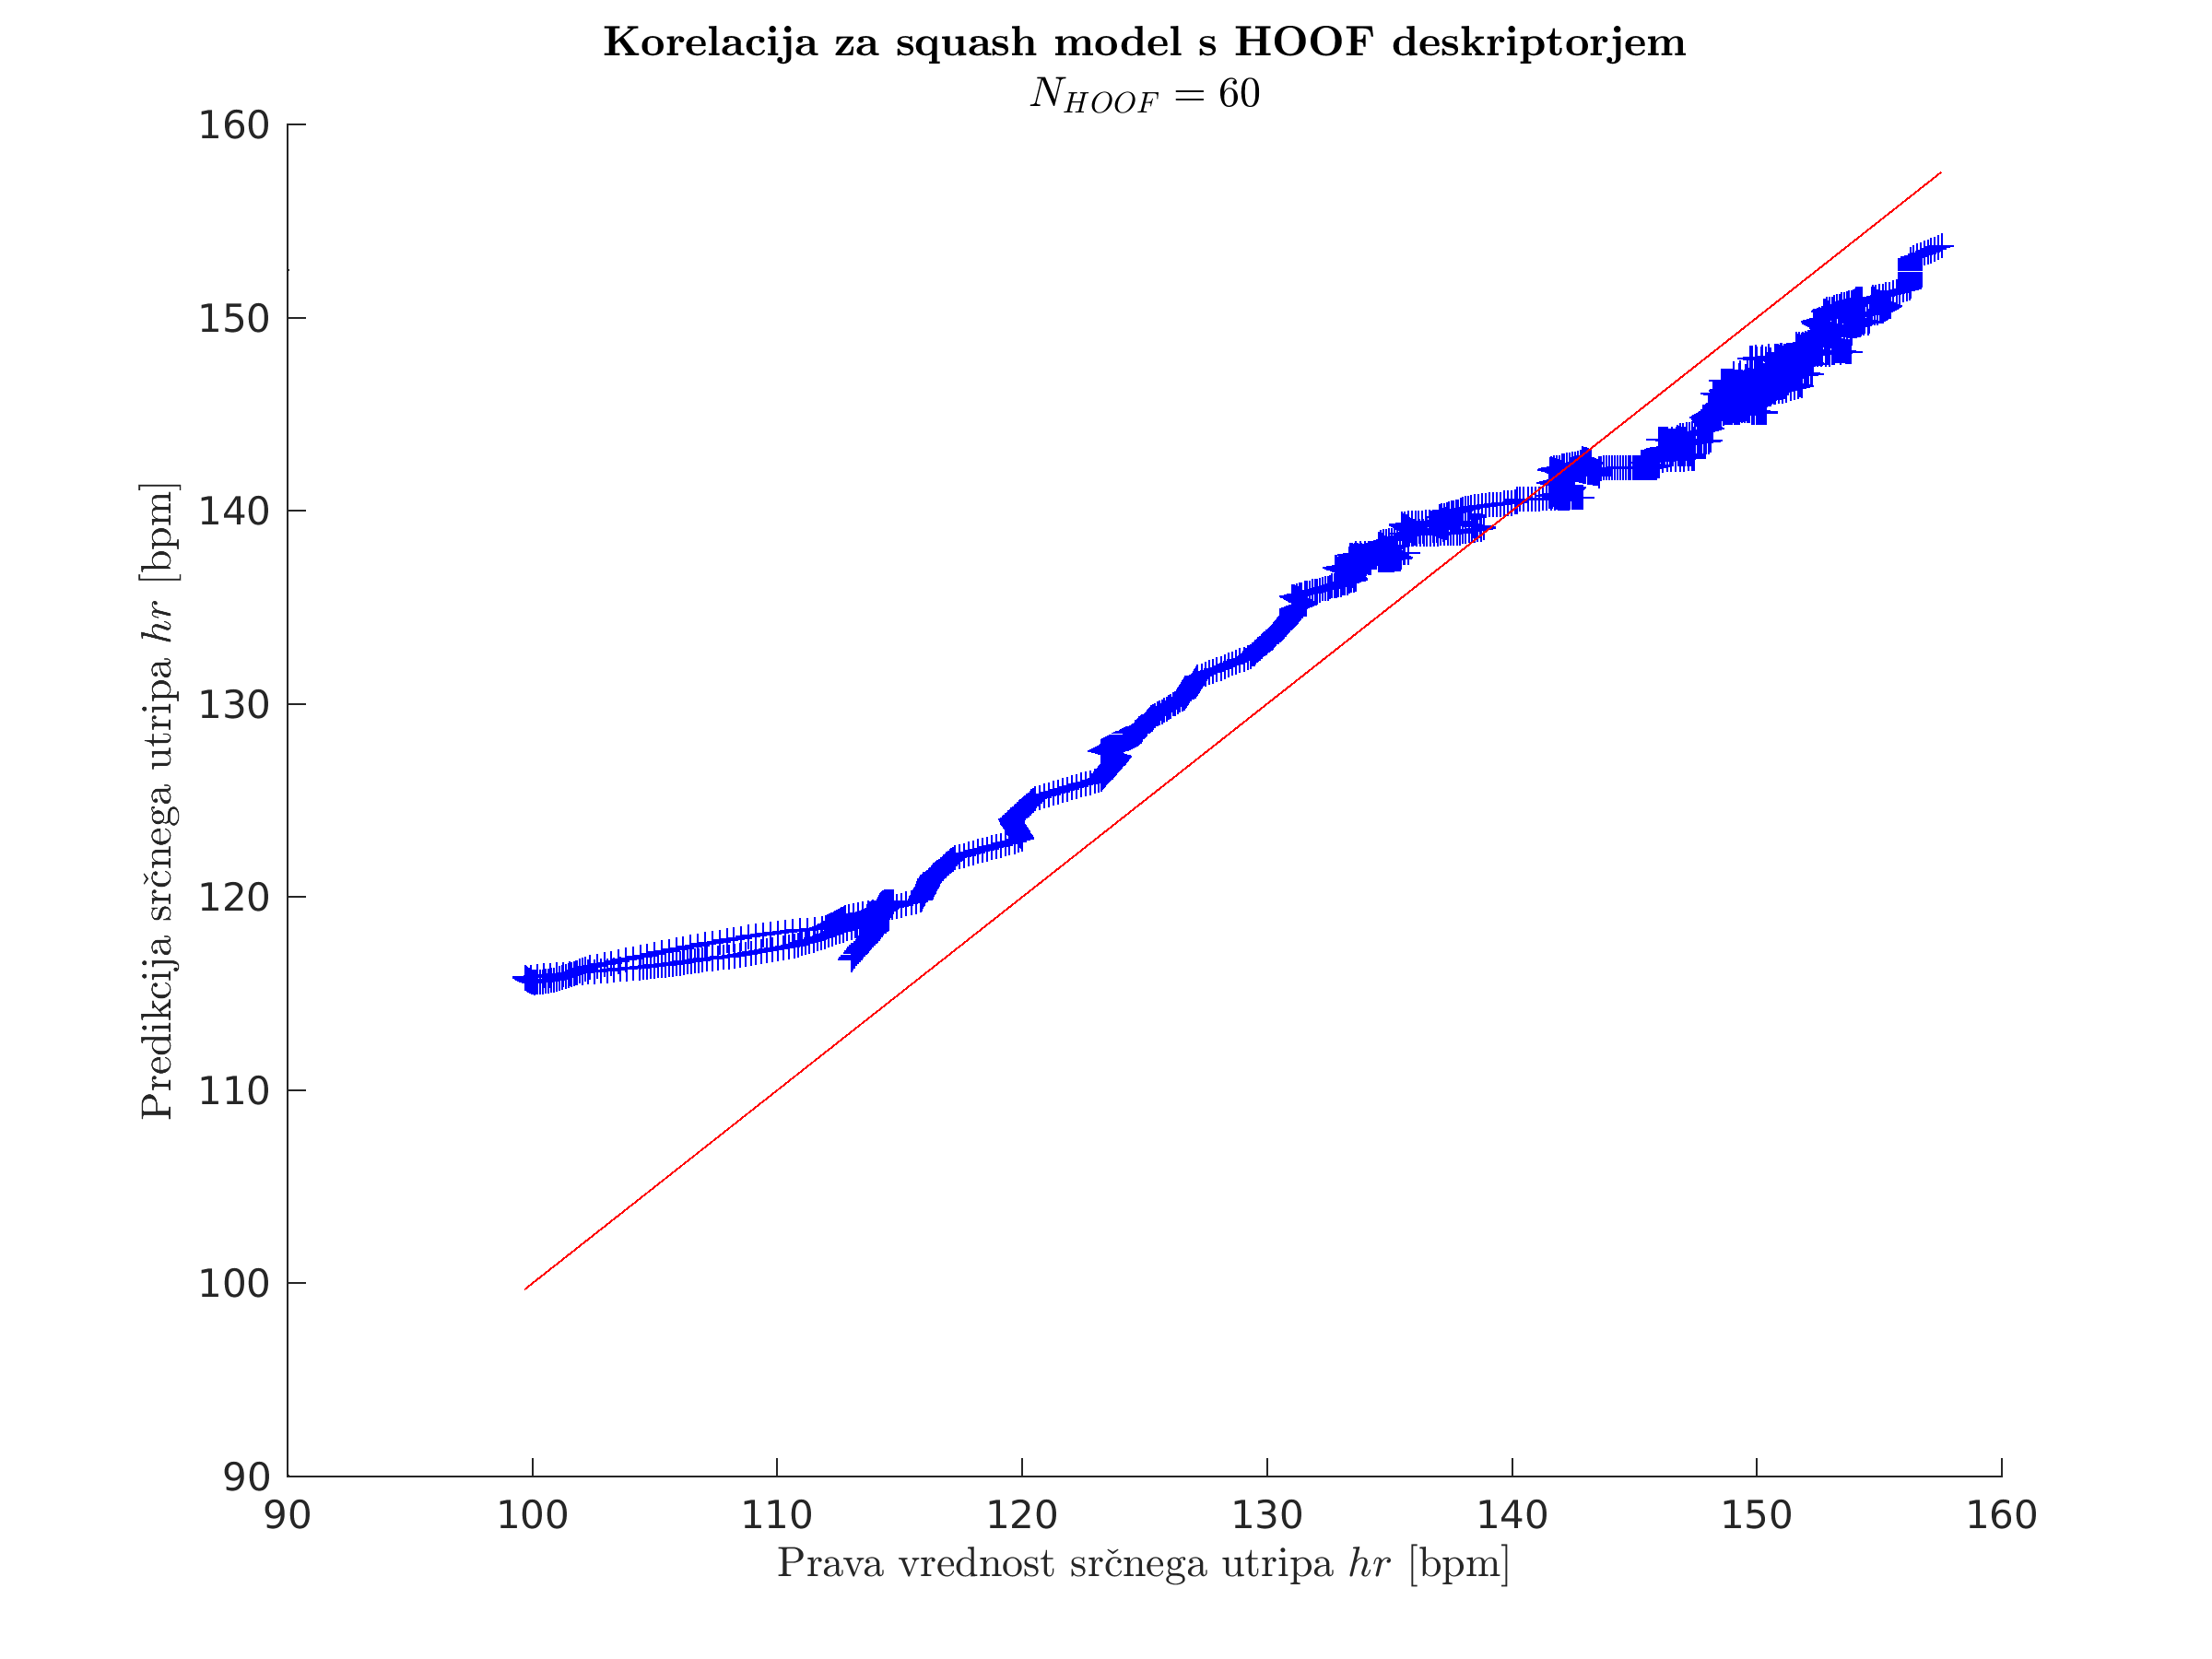
\includegraphics[width=\columnwidth]{./Slike/corr-hoof.png}
		\caption{Korelacija $N_{HOOF}=60$.}
		\label{fig:izbira-hoof}
	\end{subfigure}
	~
	\begin{subfigure}[t]{0.45\columnwidth}
		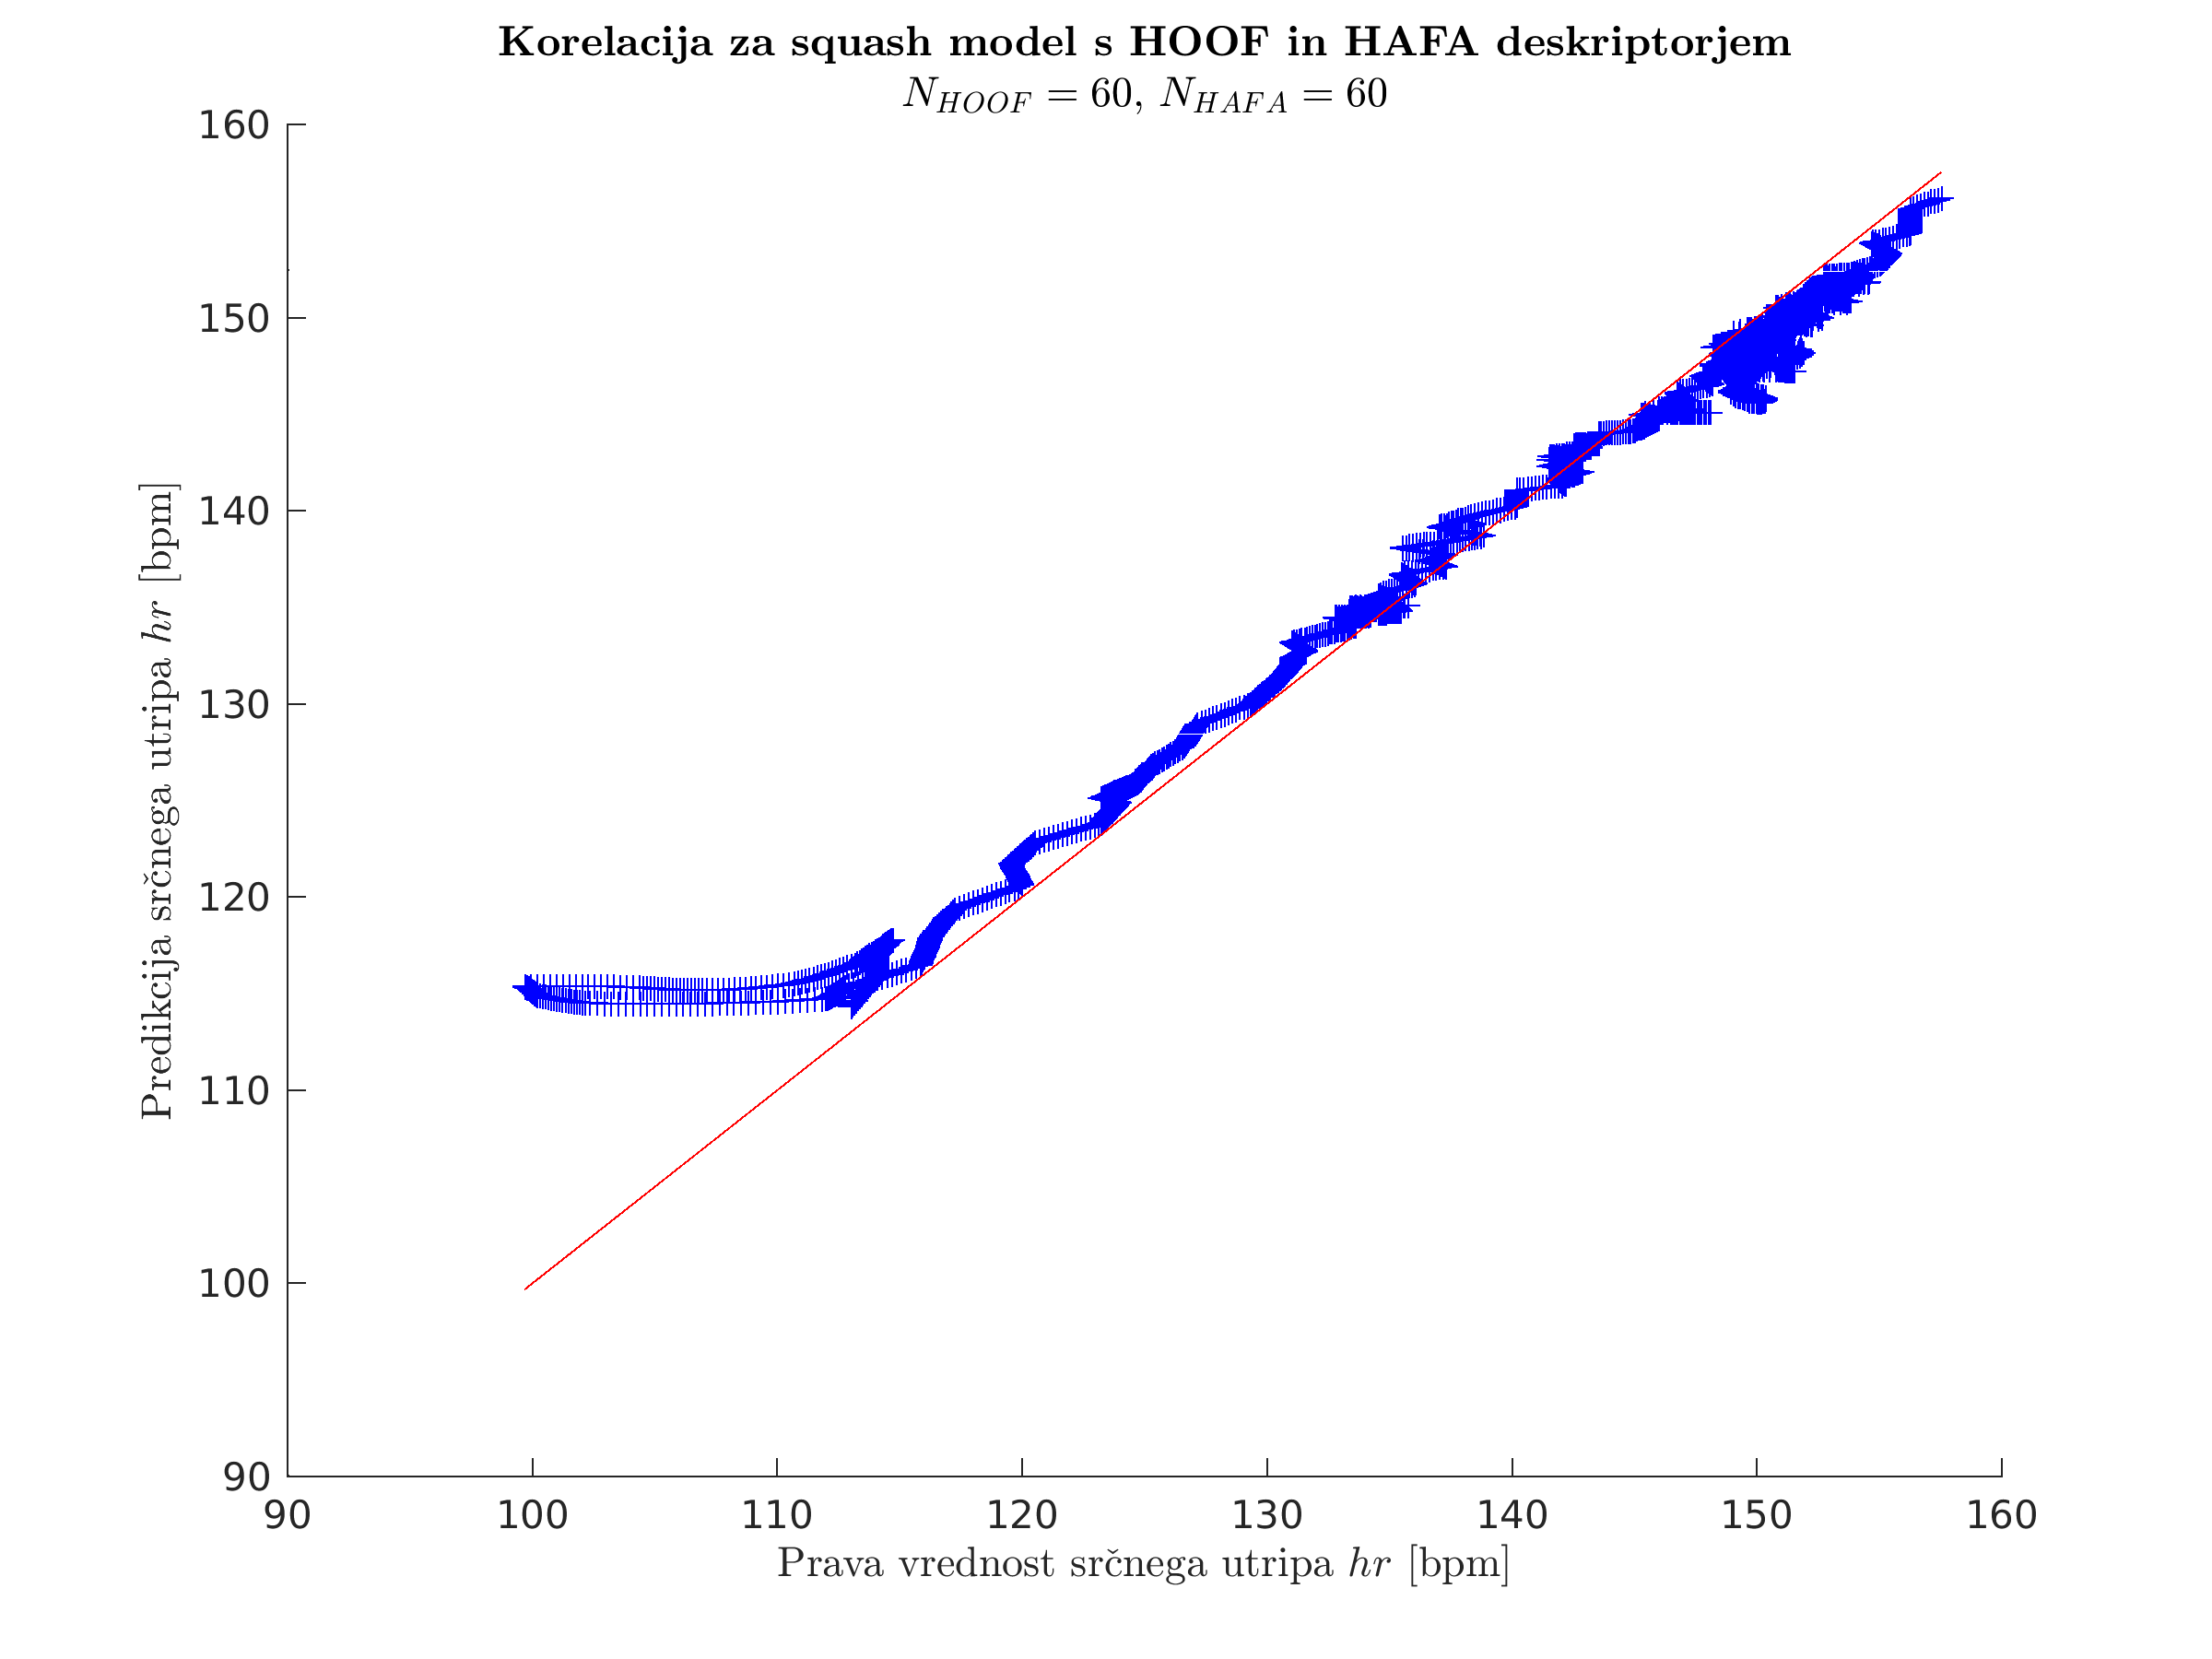
\includegraphics[width=\columnwidth]{./Slike/corr-hoof-hafa.png}
		\caption{Korelacija $N_{HOOF}=60$,\\$N_{HAFA}=60$.}
		\label{fig:izbira-hoofhafa}
	\end{subfigure}
	\caption[Primerjava modelov s HOOF in HOOF-HAFA deskriptorji]{Primerjava grafov korelacij modelov z različnimi deskriptorji. Model \subref{fig:izbira-hoof}) smo naučili s HOOF deskriptorjem. Model \subref{fig:izbira-hoofhafa}) smo naučili s HOOF in HAFA deskriptorjem. Posamezen vzorec je tako vseboval $120$ značilk. Pri primerjavi korelacije lahko opazimo vidno razliko. Model \subref{fig:izbira-hoofhafa}) dokazuje, da je razširjeni deskriptor boljši.}
	\label{fig:izbira}
\end{figure}




















\subsubsection{Sledilniki za optični tok} \label{sec:rezultati-sledilnikov-za-opticni-tok}


Rezultati testiranja so prikazani v tabeli \ref{tab:region-overlap}. Za izbrane sledilnike smo določili povprečje prekrivanja področja za posamezen posnetek. V tretjem stolpcu je predstavljeno povprečje prekrivanja glede na oba posnetka. Najboljši rezultati so odebeljeni. Po tabeli \ref{tab:region-overlap} se za posnetek \textit{handball1} najbolje izkaže CORR sledilnik. Za posnetek \textit{handball2} smo dobili najboljše rezultate pri sledilniku OPENCV-TLD. V povprečju se najbolje izkaže sledilnik CORR.




\begin{table}[htb]
	\centering
	\begin{tabular}{l S[table-format=1.3] S[table-format=1.3] S[table-format=1.3]}
		\toprule
		\textbf{Sledilnik} & \thead{$\mathbf{\Phi(\mathrm{handball1})}$} & \thead{$\mathbf{\Phi(\mathrm{handball2})}$} & \thead{$\mathbf{\overline{\Phi}}$}  \\
		\midrule%nSV
		NEBEHAY-TLD & 0.035 & 0.130 & 0.083 \\
		CCV-TLD & 0.117 & 0 & 0.117 \\
		OPENCV-TLD & 0.002 & \boldentry{1.3}{0.178} & 0.09 \\
		CORR & \boldentry{1.3}{0.214} & 0.160 & \boldentry{1.3}{0.187} \\
		\textbf{KCF} & {0.161} & {0.166} & {0.164} \\
		\bottomrule
	\end{tabular}
	\caption[Povprečje prekrivanja področja za posamezen sledilnik]{Povprečje prekrivanja področja za posamezen sledilnik in posnetek. V tretjem stolpcu je predstavljeno povprečje prekrivanja glede na oba posnetka. Najboljši rezultati so odebeljeni. Po tabeli \ref{tab:region-overlap} se za posnetek \textit{handball1} najbolje izkaže CORR sledilnik. Za posnetek \textit{handball2} smo dobili najboljše rezultate pri sledilniku OPENCV-TLD. V povprečju se najbolje izkaže sledilnik CORR.}
	\label{tab:region-overlap}
\end{table}


Na sliki \ref{fig:tracker-visual} lahko vidimo primer delovanja sledilnikov za oba posnetka. Referenčni igralec, ki mu morajo slediti ima rumeno majico. Za posnetek \textit{handball1} je predstavljena 15. slika, za posnetek \textit{handball2} pa 111. slika. Rezultati v tabeli \ref{tab:region-overlap} se skladajo z opažanji na sliki \ref{fig:tracker-visual}.

\begin{figure}[!htbp]
	\centering
	
	\begin{subfigure}[t]{0.45\columnwidth}
		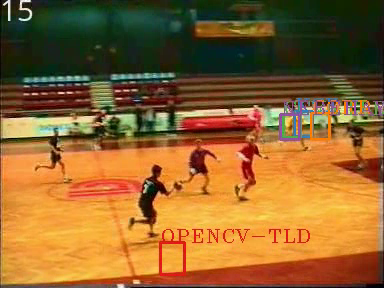
\includegraphics[width=\columnwidth]{./Slike/handball1-example.png}
		\caption{15. slika posnetka \textit{handball1}.}
		\label{fig:handball1}
	\end{subfigure}
	~
	\begin{subfigure}[t]{0.45\columnwidth}
		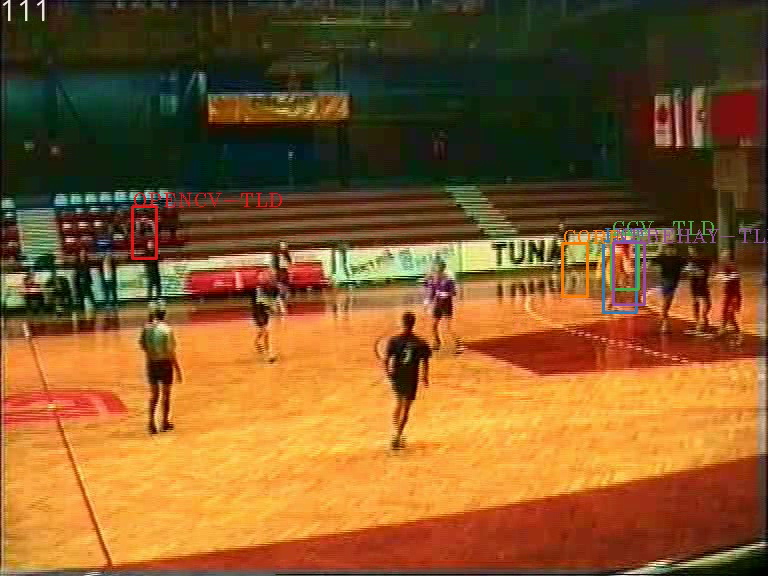
\includegraphics[width=\columnwidth]{./Slike/handball2-example.png}
		\caption{111. slika posnetka \textit{handball2}.}
		\label{fig:handball2}
	\end{subfigure}  
	\caption[Primer delovanja sledilnikov za \textit{handball} posnetke]{Primer delovanja sledilnikov za \textit{handball} posnetke. Referenčni igralec, ki mu morajo slediti ima rumeno majico. }
	\label{fig:tracker-visual}
\end{figure}




Čeprav smo z mero določili, da se je najbolje izkazal sledilnik CORR, se je pri hitri vizualni oceni sledenja na izsekih posnetka \cite{squashtv2014squash} izkazalo, da najbolje deluje sledilnik KCF. Primer boljšega delovanja KCF sledilnika je slika \ref{fig:squash-tracker-visual}, kjer sledimo modremu igralcu. Na isti sliki posnetka je KCF algoritem našel modrega igralca, medtem ko ga je CORR algoritem zamenjal z drugim igralcem. 



\begin{figure}[!htbp]
	\centering
	
	\begin{subfigure}[t]{0.45\columnwidth}
		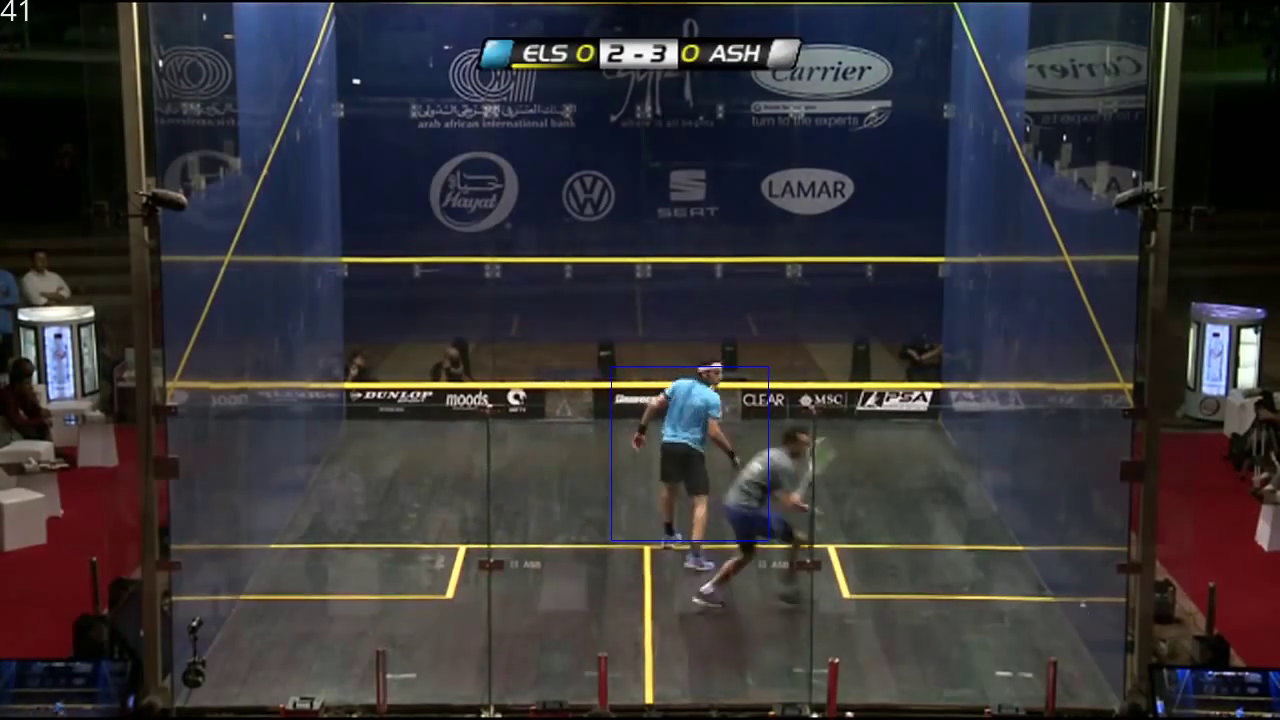
\includegraphics[width=\columnwidth]{./Slike/squash-1-kcf-example.png}
		\caption{41. slika posnetka \cite{squashtv2014squash} s KCF sledilnikom.}
		\label{fig:squash-1-kcf}
	\end{subfigure}
	~
	\begin{subfigure}[t]{0.45\columnwidth}
		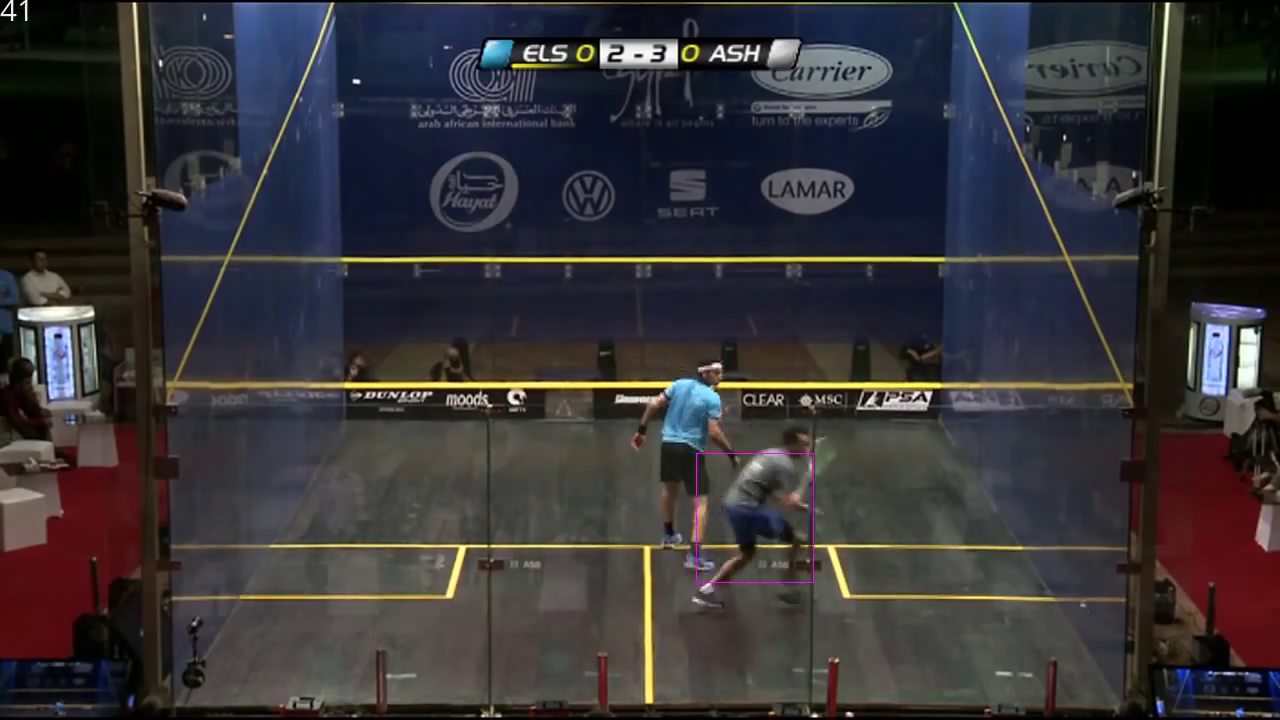
\includegraphics[width=\columnwidth]{./Slike/squash-1-corr-example.png}
		\caption{41. slika posnetka \cite{squashtv2014squash} s CORR sledilnikom.}
		\label{fig:squash-1-corr}
	\end{subfigure}  
	\caption[Primer delovanja sledilnikov za squash posnetek]{Primer delovanja sledilnikov za squash posnetek. Gre za identični sliki posnetka, pri čemer smo na sliki \ref{fig:squash-1-kcf} uporabili KCF algoritem, na sliki \ref{fig:squash-1-corr} pa CORR algoritem. Sledilnika sta morala slediti igralcu z modro majico.}
	\label{fig:squash-tracker-visual}
\end{figure}


Boljše delovanje KCF je razumljivo, saj prvi testi temeljijo na posnetkih rokometa, drugi pa na squashu, kjer gre za bistveno drugačno igro. Če pogledamo tabelo \ref{tab:region-overlap} ima KCF drugo najboljše povprečje, prav tako pa so si rezultati posameznih posnetkov zelo podobni. 


















\subsection{Elementarni eksperimenti tekalne steze}
As can be seen in the Table \ref{tab:initial-models-validation}, we get relatively poor results in the prediction of heart rate.

\begin{table}[!htb]
	\centering
	{\footnotesize
      \begin{tabular}{l S[table-format=3.2, detect-weight, detect-shape, detect-mode] S[table-format=3.2, detect-weight, detect-shape, detect-mode] S[table-format=3.2, detect-weight, detect-shape, detect-mode]}
          \toprule
          \textbf{Model} & \multicolumn{1}{c}{\textbf{CORR}} & \multicolumn{1}{c}	{\textbf{RAE} (\%)} & \multicolumn{1}{c}{\textbf{RRSE} (\%)} \\
          \midrule
          hr-sv(sv) & 0.90 & 75.42 & 76.66	\\
          hr-sv(bv)	&	-0.66	&	104.61	&	110.17	\\
\bfseries hr-sv-lag(sv)		&	\bfseries 0.93	&	\bfseries 74.37	&	\bfseries 75.51	\\
          hr-sv-lag(bv)	&	-0.87	&	138.60	&	136.62	\\
          hr-bv(sv)	&	0.83	&	311.95	&	295.66	\\
          hr-bv(bv)	 	&	0.88	&	81.07	&	79.27	\\
          hr-bv-lag(sv)	&	0.49	&	84.71	&	89.40	\\
          hr-bv-lag(bv) 	&	0.91	&	79.15	&	76.93	\\
          eem-sv(sv)		&	0.87	&	47.08	&	49.75	\\
          eem-sv(bv)	&	-0.75	&	109.27	&	117.62	\\
          \bfseries eem-sv-lag(sv)	&	\bfseries 0.92	&	\bfseries 38.15	&	\bfseries 40.18	\\
          eem-sv-lag(bv)	&	-0.74	&	121.86	&	121.88	\\
          eem-bv(sv)	&	0.61	&	94.92	&	95.92	\\
          eem-bv(bv)		&	0.85	&	44.51	&	56.24	\\
          eem-bv-lag(sv)	&	0.86	&	56.60	&	68.61	\\
          eem-bv-lag(bv)	&	0.90	&	45.51	&	49.50	\\
          \bottomrule        
      \end{tabular}
	}
	\caption{The results of the initial model evaluations with cross testing. For each model, we calculated the correlation coefficient (CORR), relative absolute error (RAE) and root relative square error (RRSE).}
	\label{tab:initial-models-validation}
\end{table}

In terms of using different view angles, we get best results for side-view. We assume that this is due to the fact that with a back-view camera (without any cropping) we also recorded the movement of the operator, who is not visible in side-view recordings. Despite the fact that the HOOF features get rid of the noise of the optical flow, the movement of the operator is intensive enough to be able to influence the results. Worse results for back-view camera could also indicate that we get less descriptive features from it. 
%V smislu uporabe različnih zornih kotov, smo dobili najboljše rezultate pri stranskem pogledu. Predvidevamo, da je to posledica dejstva, da smo s kamero pri hrbtnem pogledu snemali tudi gibanje operaterja, česar pa v stranskem pogledu ni. Kljub dejstvu, da se s HOOF značilkami znebimo šuma optičnega toka, je gibanje operaterja dovolj intenzivno, da bi lahko vplivalo na rezultat.

The results of the models, where we assume the delay between excitation and response are better, which indicates that the assumption is justified.
%Rezultati modelov, kjer smo predpostavili časovni zamik med vzbujanjem in odzivom so boljši, kar nakazuje na to, da je predpostavka upravičena.

Considering cross testing we can see, that all models produce poorer results if we test them with data from different viewing angle.

The best results were obtained in the prediction of the energy expenditure (EEM). Output signals of the best results for the prediction of energy expenditure and heart rate are presented in Figure \ref{fig:rezultat}. The curves of the results have the same form because they are correlated physiological parameters.
%Najboljši rezultat smo dobili pri predikciji hitrosti porabe energije (EEm). Izhodni signali najboljših rezultatov za predikcijo energijske porabe in srčnega utripa so predstavljeni na sliki \ref{fig:rezultat}.

\begin{figure}[!htb]
	\centering
    %\includegraphics[width=0.9\linewidth]{./slike/best-results.eps}
    \caption{The best results for prediction of energy expenditure and heart rate when validating the models. The figure shows the output of models eem-sv-lag(sv) and hr-sv-lag(sv) and the actual value of energy expenditure and heart rate.}
    %\caption{Najboljša rezultata za predikcijo porabe energije in srčnega utripa pri validaciji modelov. Slika prikazuje izhod modelov eem-sv-l in hr-sv-l ter dejanske vrednosti hitrosti porabe energije na minuto in srčnega utripa.}
    \label{fig:rezultat}
\end{figure}















\subsection{Ročna določitev področja zanimanja}
















\subsection{Eksperimenti združenih posnetkov}
As in initial models, when comparing models with different physiological parameters in Table \ref{tab:mixed-models-validation}, heart rate models produce worse results. Lag models are better than normal models and best result is still produced by lagged model, which predicts energy expenditure.

\begin{table}[!htb]
	\centering
	{\footnotesize
      \begin{tabular}{l  S[table-format=3.2, detect-weight, detect-shape, detect-mode]  S[table-format=3.2, detect-weight, detect-shape, detect-mode]  S[table-format=3.2, detect-weight, detect-shape, detect-mode]}
          \toprule
          \textbf{Model} & \multicolumn{1}{c}{\textbf{CORR}} & \multicolumn{1}{c}	{\textbf{RAE} (\%)} & \multicolumn{1}{c}{\textbf{RRSE} (\%)} \\
          \midrule
        hr-mixed(sv)	&	0.89	&	67.18	&	68.17	\\
        hr-mixed(bv)	&	0.88	&	59.84	&	61.89	\\
        hr-mixed-lag(sv) &	0.92	&	65.24	&	66.44	\\
        \bfseries hr-mixed-lag(bv) &	\bfseries 0.91	&	\bfseries 57.75	&	\bfseries 60.31	\\
        eem-mixed(sv)	&	0.85	&	45.90	&	53.89	\\
        eem-mixed(bv)	&	0.84	&	57.44	&	62.78	\\
        \bfseries eem-mixed-lag(sv)	&	\bfseries 0.90	&	\bfseries 44.19	&	\bfseries 46.09	\\
        eem-mixed-lag(bv)	&	0.89	&	56.70	&	55.04	\\
          \bottomrule        
      \end{tabular}
	}
	\caption{The results of the mixed model evaluations with cross testing. For each model, we calculated the correlation coefficient (CORR), relative absolute error (RAE) and root relative square error (RRSE).}
	\label{tab:mixed-models-validation}
\end{table}

The main difference in mixed models can be seen, when comparing cross tests. If we compare results from Table \ref{tab:initial-models-validation} and \ref{tab:mixed-models-validation}, we can see that results, when testing models with data from different viewing angle as they were trained, are significantly better. This results indicate that better models could be trained with recordings from different viewing angle.













\subsection{Obremenitveni testi}















\subsection{Tekalna steza s sledenjem}
Results of models with enabled tracker are represented in Table \ref{tab:tracker-models-validation}. If we compare them with results of initial models in Table \ref{tab:initial-models-validation}, the mean absolute difference of RRSE between them is \SI{28}{\%}. We can assume that this is due to the fact that tracker does not track selected object perfectly. In some cases it cannot find object, or detects wrong object. It can also track only part of the object. This anomalies can affect calculation of physiological parameters.

\begin{table}[!htb]
	\centering
	{\footnotesize
      \begin{tabular}{l S[table-format=3.2, detect-weight, detect-shape, detect-mode] S[table-format=3.2, detect-weight, detect-shape, detect-mode] S[table-format=3.2, detect-weight, detect-shape, detect-mode]}
          \toprule
          \textbf{Model} & \multicolumn{1}{c}{\textbf{CORR}} & \multicolumn{1}{c}	{\textbf{RAE} (\%)} & \multicolumn{1}{c}{\textbf{RRSE} (\%)} \\
          \midrule
        hr-sv-tr(sv)	&	0.93	&	90.82	&	86.55	\\
        hr-sv-tr(bv)	&	-0.18	&	133.17	&	145.74	\\
        \bfseries hr-sv-lag-tr(sv)	&	\bfseries 0.96	&	\bfseries 91.57	&	\bfseries 86.72	\\
        hr-sv-lag-tr(bv)	&	-0.11	&	108.99	&	124.40	\\
        hr-bv-tr(sv)	&	-0.55	&	132.25	&	146.66	\\
        hr-bv-tr(bv)	&	0.89	&	116.38	&	111.78	\\
        hr-bv-lag-tr(sv)	&	-0.62	&	131.09	&	140.59	\\
        hr-bv-lag-tr(bv)	&	0.91	&	118.69	&	113.24	\\
        eem-sv-tr(sv)	&	0.90	&	41.55	&	45.25	\\
        eem-sv-tr(bv)	&	-0.34	&	135.25	&	141.63	\\
        \bfseries eem-sv-lag-tr(sv)	&	\bfseries 0.94	&	\bfseries 31.66	&	\bfseries 37.05	\\
        eem-sv-lag-tr(bv)	&	0.65	&	126.00	&	130.04	\\
        eem-bv-tr(sv)	&	-0.44	&	107.47	&	107.91	\\
        eem-bv-tr(bv)	&	0.91	&	53.21	&	52.92	\\
        eem-bv-lag-tr(sv)	&	-0.68	&	110.55	&	113.64	\\
        eem-bv-lag-tr(bv)	&	0.93	&	41.57	&	51.53	\\
        hr-sv-tr-sh(sv)	&	0.92	&	90.39	&	87.15	\\
        hr-sv-tr-sh(bv)	&	0.84	&	90.98	&	112.00 \\
        \bfseries hr-sv-lag-tr-sh(sv)	&	\bfseries 0.95	&	\bfseries 88.86 	&	\bfseries 86.99	\\
        hr-sv-lag-tr-sh(bv)	&	-0.10	&	111.46	&	118.79	\\
        hr-bv-tr-sh(sv)	&	0.83	&	286.16	&	268.48	\\
        hr-bv-tr-sh(bv)	&	0.87	&	113.11	&	111.15	\\
        hr-bv-lag-tr-sh(sv)	&	0.89	&	293.45	&	275.83	\\
        hr-bv-lag-tr-sh(bv)	&	0.87	&	114.98	&	113.90	\\
        eem-sv-tr-sh(sv)	&	0.90	&	50.18	&	59.92	\\
        eem-sv-tr-sh(bv)	&	0.89	&	119.57	&	128.17	\\
        eem-sv-lag-tr-sh(sv)	&	0.93	&	51.47	&	56.55	\\
        eem-sv-lag-tr-sh(bv)	&	-0.08	&	135.85	&	133.27	\\
        eem-bv-tr-sh(sv)	&	0.75	&	179.11	&	172.30	\\
        eem-bv-tr-sh(bv)	&	0.90	&	52.85	&	54.43	\\
        eem-bv-lag-tr-sh(sv)	&	0.91	&	175.29	&	171.63	\\
        \bfseries eem-bv-lag-tr-sh(bv)	&	\bfseries 0.94	&	\bfseries 50.02	&	\bfseries 48.93	\\
          \bottomrule        
      \end{tabular}
	}
	\caption{The results of the tracker model evaluations with cross testing. For each model, we calculated the correlation coefficient (CORR), relative absolute error (RAE) and root relative square error (RRSE).}
	\label{tab:tracker-models-validation}
\end{table}

The mean absolute difference of RRSE between normal tracking models and models with shaking video is about \SI{30}{\%}. Results are worse with videos that incorporate shaking (motion noise), but this is still acceptable, because the selected tracker can stabilize our video and improve results.















\subsection{Simulacija vibracij kamere}












\subsection{Terenski eksperimenti squash igre}
If we compare Table \ref{tab:initial-models-validation} and Table \ref{tab:squash-models-validation}, we can see that result for squash model is not far behind one of the best results in initial models, despite the fact that we used different subjects for training and testing. 

\begin{table}[!htb]
	\centering
	{\small
      \begin{tabular}{l D{.}{.}{-1} D{.}{.}{-1} D{.}{.}{-1}}
          \toprule
          \textbf{Model} & \multicolumn{1}{c}{\textbf{CORR}} & \multicolumn{1}{c}	{\textbf{RAE} (\%)} & \multicolumn{1}{c}{\textbf{RRSE} (\%)} \\
          \midrule
        hr-bv-lag-tr-sq	&	0.45	&	68.65	&	54.24	\\
          \bottomrule        
      \end{tabular}
	}
	\caption{The results of the squash match evaluation. For model, we calculated the correlation coefficient (CORR), relative absolute error (RAE) and root relative square error (RRSE).}
	\label{tab:squash-models-validation}
\end{table}

If we further explore our model from realistic data, we can see in Figure \ref{fig:squash-result} that predicted working point is about \SI{7}{bpm} lower. The reason could be that training data is extracted only from one subject. The second reason could be imperfections of used equation from \cite{charlot2014improvement}. Despite these errors a coarse prediction is still possible, even if we don't train the algorithm on the same subject.

% Razlaga rezultatov je, da so vredu, le delovna točka je faljena zaradi majhne variacije učnih vzorcev (učimo namreč le na eni osebi) in pa nenatančnosti same enačbe, ki jo uporabljamo za pretvorbo. Če učimo z eno osebo in probamo na drugi osebi ji lahko napovemo srčni utrip s cca. 7 bpm napake

\begin{figure}[!htb]
	\centering
    %\includegraphics[width=0.9\linewidth]{./slike/squash-result.eps}
    \caption{Result for prediction of heart rate when validating the models. The figure shows the output of model hr-bv-lag-tr-sq and the actual value of heart rate.}
    \label{fig:squash-result}
\end{figure}






















\subsection{Eksperiment detekcije dihanja}

For breathing detection, which was formulated as a classification problem, we used standard metrics for evaluation of two-class classification problems. With ''breathing'' considered the ''true'' value, and ''not breathing'' the ''false'' we get the following results: false positive rate, FPR = \SI{13}{\%}, true positive rate, TPR = \SI{87}{\%}, false negative rate, FNR = \SI{26}{\%}, true negative rate, TNR = \SI{74}{\%}.































\section{Eksperimenti 2. faze}










\subsection{Preliminarni eksperimenti}





\subsubsection{Združevanje slik iz dveh Kinect kamer}\label{sec:rezultati-zdruzevanje}
Združevanje s značilkami se ni obneslo, zato smo to metodo opustili. Primer neuspelega poskusa je prikazan na sliki \ref{fig:zdruzevanje-znacilke}.

\begin{figure}[!htb]
	\centering
	\begin{subfigure}[t]{0.45\columnwidth}
		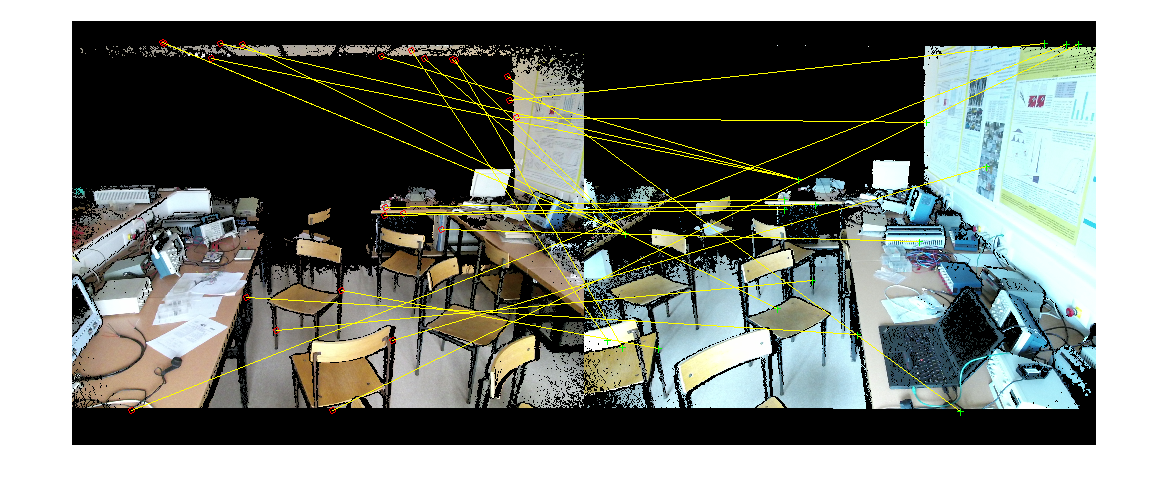
\includegraphics[width=\columnwidth]{./Slike/matched-features.png}
		\caption{Ujemajoče SURF značilke}
		\label{fig:zdruzevanje-surf}
	\end{subfigure}
	~
	\begin{subfigure}[t]{0.45\columnwidth}
		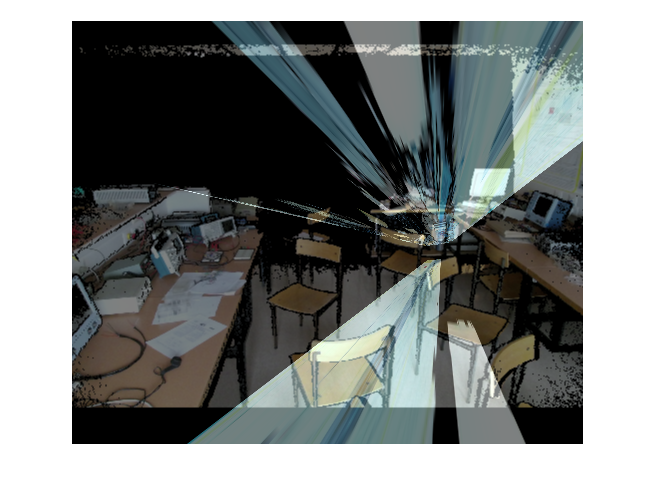
\includegraphics[width=\columnwidth]{./Slike/features-calibration-result.png}
		\caption{Rezultat združevanja z značilkami}
		\label{fig:zdruzevanje-result}
	\end{subfigure}
	\caption{Primer neuspelega poskusa združevanja slik iz dveh Kinect kamer s SURF značilkami.}
	\label{fig:zdruzevanje-znacilke}
\end{figure}

 Rezultat je bil boljši od združevanja z značilkami, vendar še vedno slab, zato smo tudi to metodo opustili. Primer neuspelega poskusa je prikazan na sliki \ref{fig:zdruzevanje-cp}.
 
 \begin{figure}[htb]
 	\centering
 	\begin{subfigure}[t]{0.45\columnwidth}
 		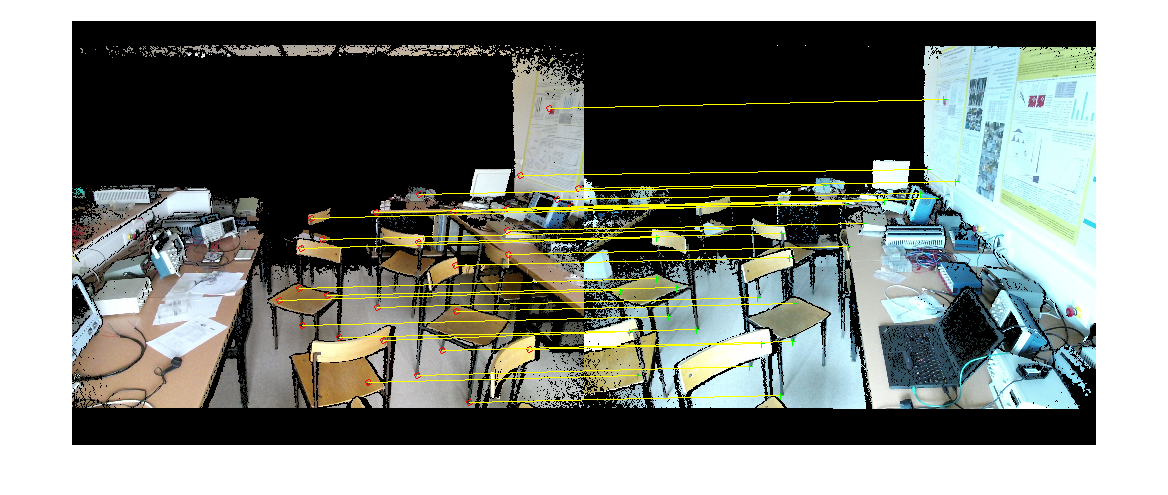
\includegraphics[width=\columnwidth]{./Slike/matched-points.png}
 		\caption{Ujemajoče kontrolne točke}
 		\label{fig:zdruzevanje-ujemajoce-cp}
 	\end{subfigure}
 	~
 	\begin{subfigure}[t]{0.45\columnwidth}
 		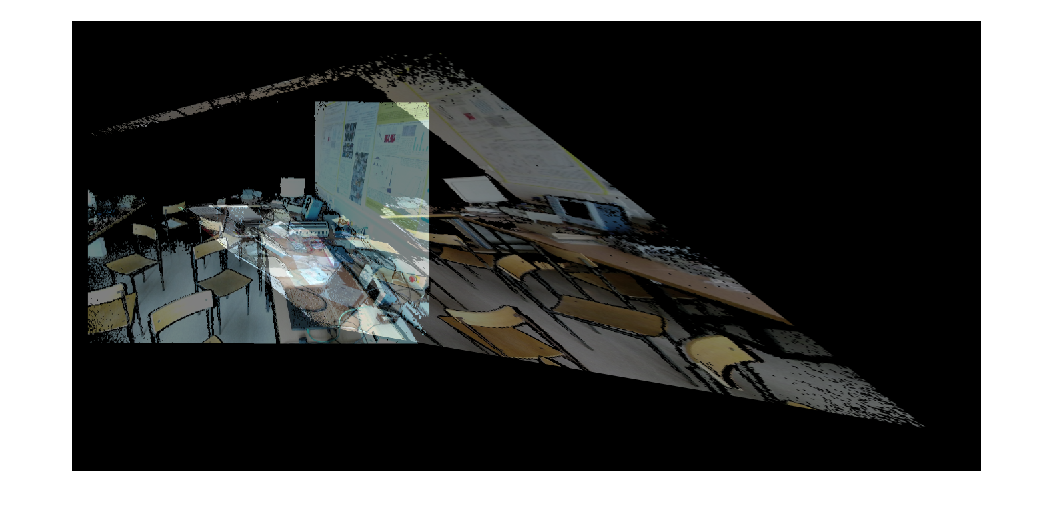
\includegraphics[width=\columnwidth]{./Slike/points-calibration-result.png}
 		\caption{Rezultat združevanja s kontrolnimi točkami}
 		\label{fig:zdruzevanje-result-cp}
 	\end{subfigure}
 	\caption{Primer neuspelega poskusa združevanja slik iz dveh Kinect kamer s kontolnimi točkami.}
 	\label{fig:zdruzevanje-cp}
 \end{figure}







\subsubsection{Optimizacija mrežnega iskanja \texorpdfstring{$\nu$}{nu}-RBF}





\subsubsection{Test mrežnega iskanja \texorpdfstring{$\nu$}{nu}-RBF}





\subsubsection{Jedro GHI}





\subsubsection{Optimizacija Gaussovega filtra}
Rezultati povrprečnih vrednosti uporabljenih metrik so vidni v tabeli \ref{tab:gauss}. Za pravilno razlago rezultatov, moramo upoštevati tudi grafe metrik posameznih eksperimentov, ki so prikazani na slikah \ref{fig:sigma1-5}, \ref{fig:sigma-rmse5-21} in \ref{fig:sigma21-51}. 



\begin{table}[htb]
	\centering
	\begin{tabular}{S[table-format=2.0] S[table-format=2.3] S[table-format=2.3]}
		\toprule
		\thead{$\mathbf{\sigma}$} & \thead{RMSE} & \thead{SNR [dB]}  \\
		\midrule%nSV
		1 & \boldentry{2.3}{8.614} & 24.278 \\
		3 & 11.236 & 25.470 \\
		\boldentry{2.0}{5} & 11.596 & 25.746 \\
		11 & 11.783 & 25.746 \\
		21 & 11.842 & 25.975 \\
		31 & 11.871 & 26.194 \\
		51 & 11.907 & \boldentry{2.3}{26.306} \\
		\bottomrule
	\end{tabular}
	\caption[Povprečne vrednosti RMSE in SNR metrik pri optimizaciji parametra $\sigma$ Gaussovega filtra]{Povprečne vrednosti RMSE in SNR metrik pri optimizaciji parametra $\sigma$ Gaussovega filtra. Najmanjši standardni odklon ima najmanjšo napako, vendar je tudi filtriranje majhno. Pri $\sigma=3$ in $\sigma=5$ so še opazne razlike pri filriranju. Za višje vrednosti ni več opazne razlike, vendar pa se napaka povečuje. $\sigma=5$ je tako optimalna vrednosti parametra.}
	\label{tab:gauss}
\end{table}

Najmanjšo napako dobimo, če uporabimo $\sigma=1$, vendar pa imamo pri tem najmanjše filtriranje, zato so rezultati še vedno lahko zelo šumni. Z višanjem parametra filtra, se napaka po metriki RMSE povečuje, vendar ima večji vpliv razmerje SNR, saj je predstavljeno v logaritemski skali. 

\begin{figure}[!htb]
	\centering
	\begin{subfigure}[t]{0.45\columnwidth}
		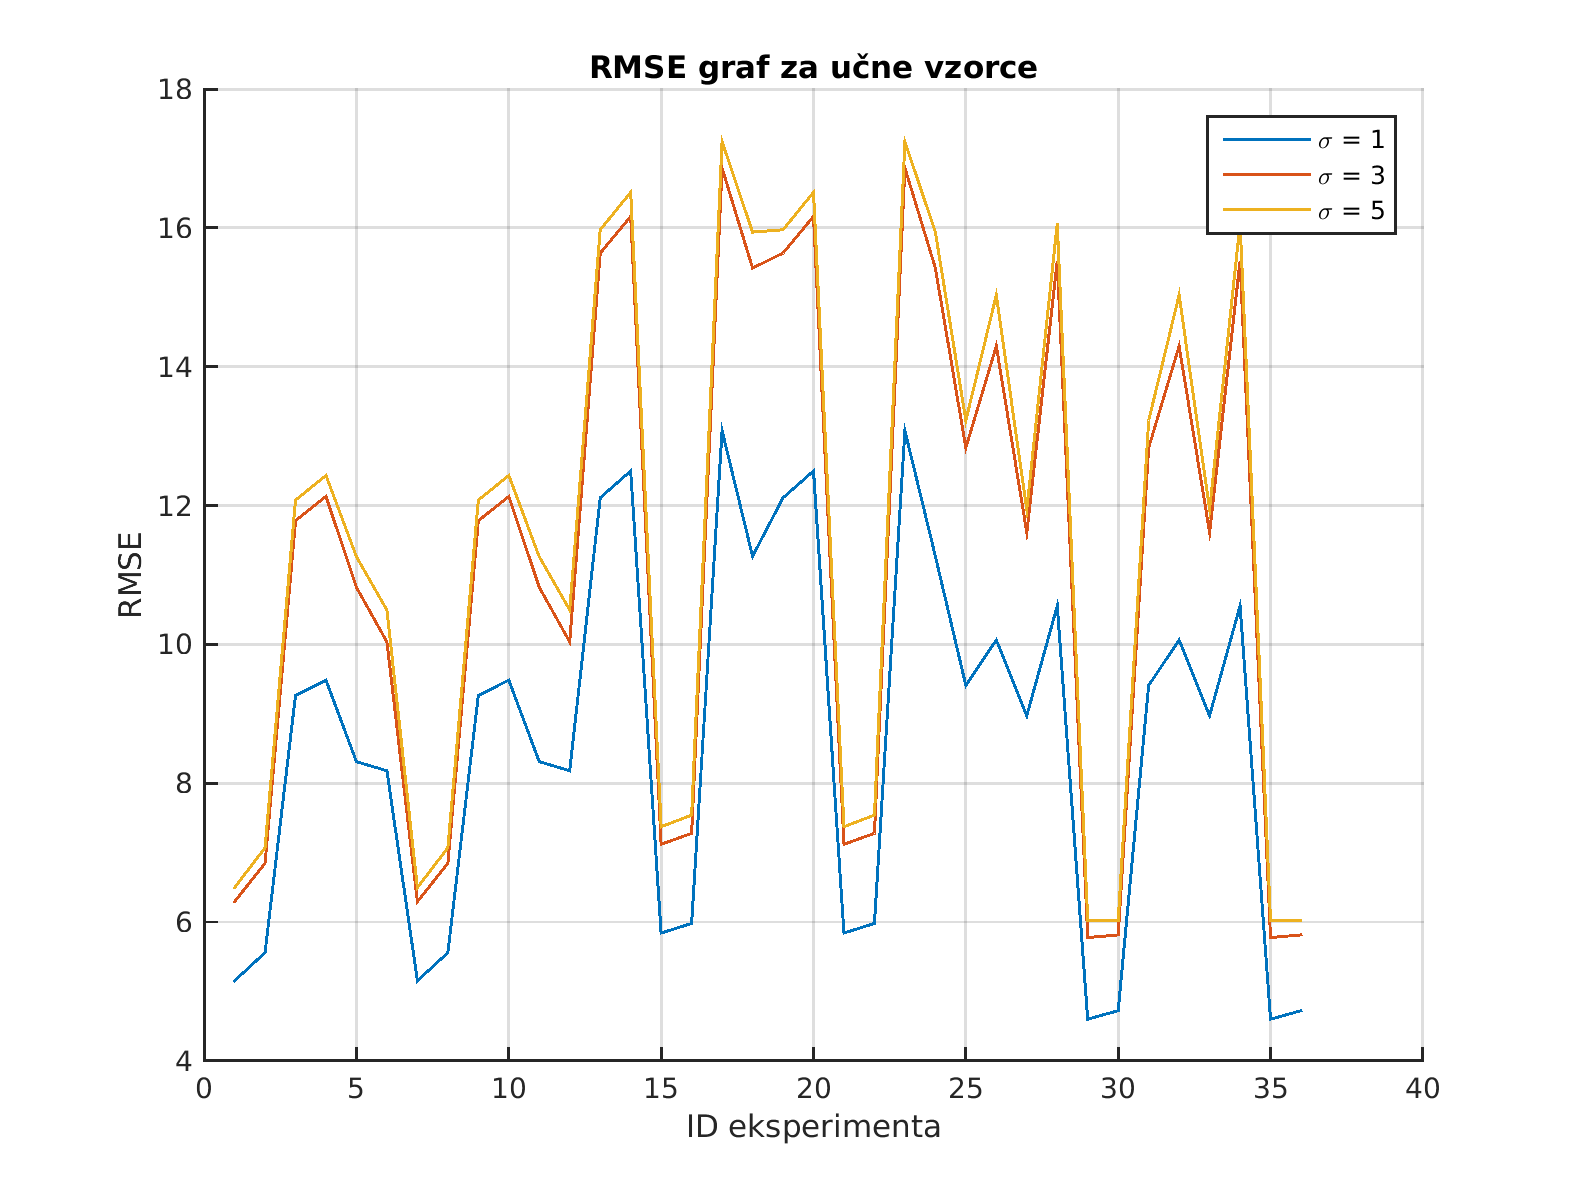
\includegraphics[width=\columnwidth]{./Slike/sigma-rmse1-5.png}
		\caption{Graf RMSE  učnih vzorcev }
		\label{fig:sigma-rmse1-5}
	\end{subfigure}
	~
	\begin{subfigure}[t]{0.45\columnwidth}
		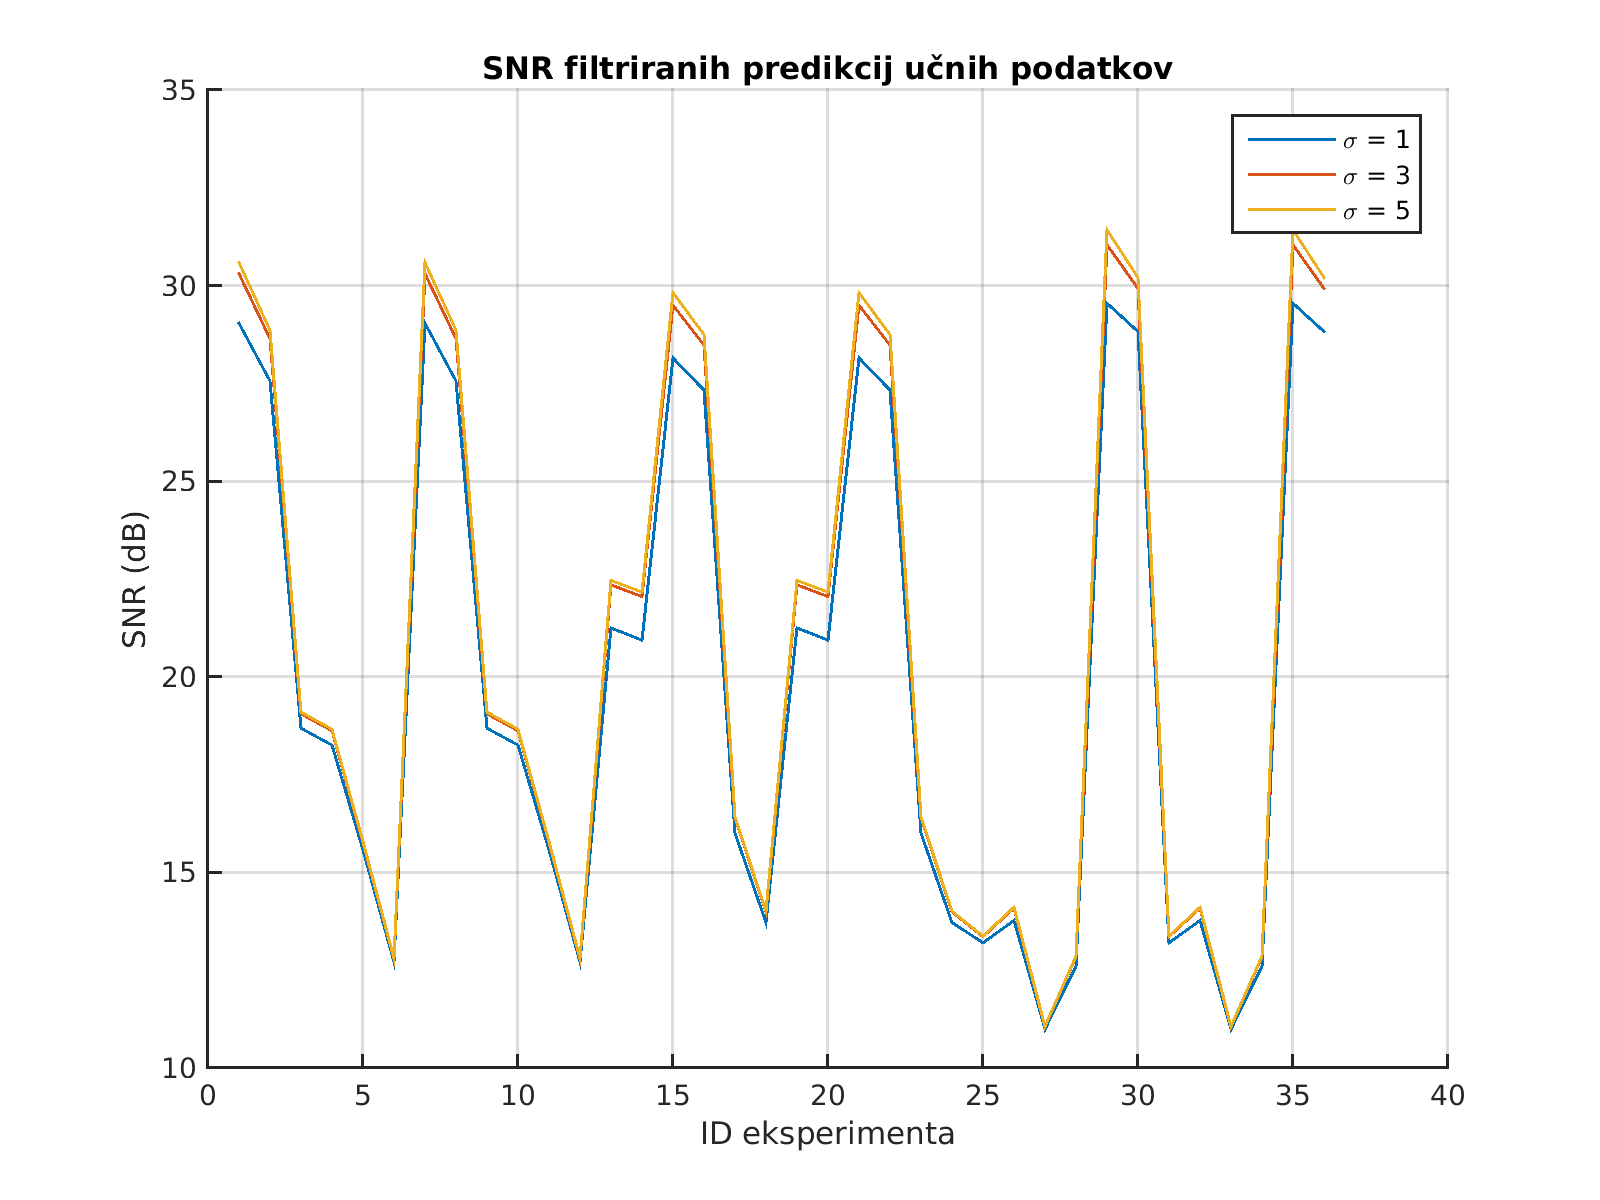
\includegraphics[width=\columnwidth]{./Slike/sigma-snr1-5.png}
		\caption{Graf SNR  učnih vzorcev}
		\label{fig:sigma-snr1-5}
	\end{subfigure}
	\caption{Grafa RMSE in SNR učnih vzorcev za \mbox{$\sigma \in [1,5]$}}
	\label{fig:sigma1-5}
\end{figure}

Čeprav pri uporabi $\sigma=51$ dobimo največje filtriranje šuma, lahko na slikah grafov opazimo, da se obe metriki bistveno ne razlikujeta za vrednosti parametra na intervalu $[5,51]$. Kljub dobremu filtriranju želimo zagotoviti čim manjšo napako med referenčnim signalom in predikcijo, zato je logična izbira čim manjši standardni odklon. Ker so na sliki \ref{fig:sigma1-5} med $\sigma=3$ in $\sigma=5$ še opazne razlike, lahko zaključimo, da je $\sigma=5$ optimalna izbira parametra za naš problem. 


\begin{figure}[htb]
	\centering
	\begin{subfigure}[t]{0.45\columnwidth}
		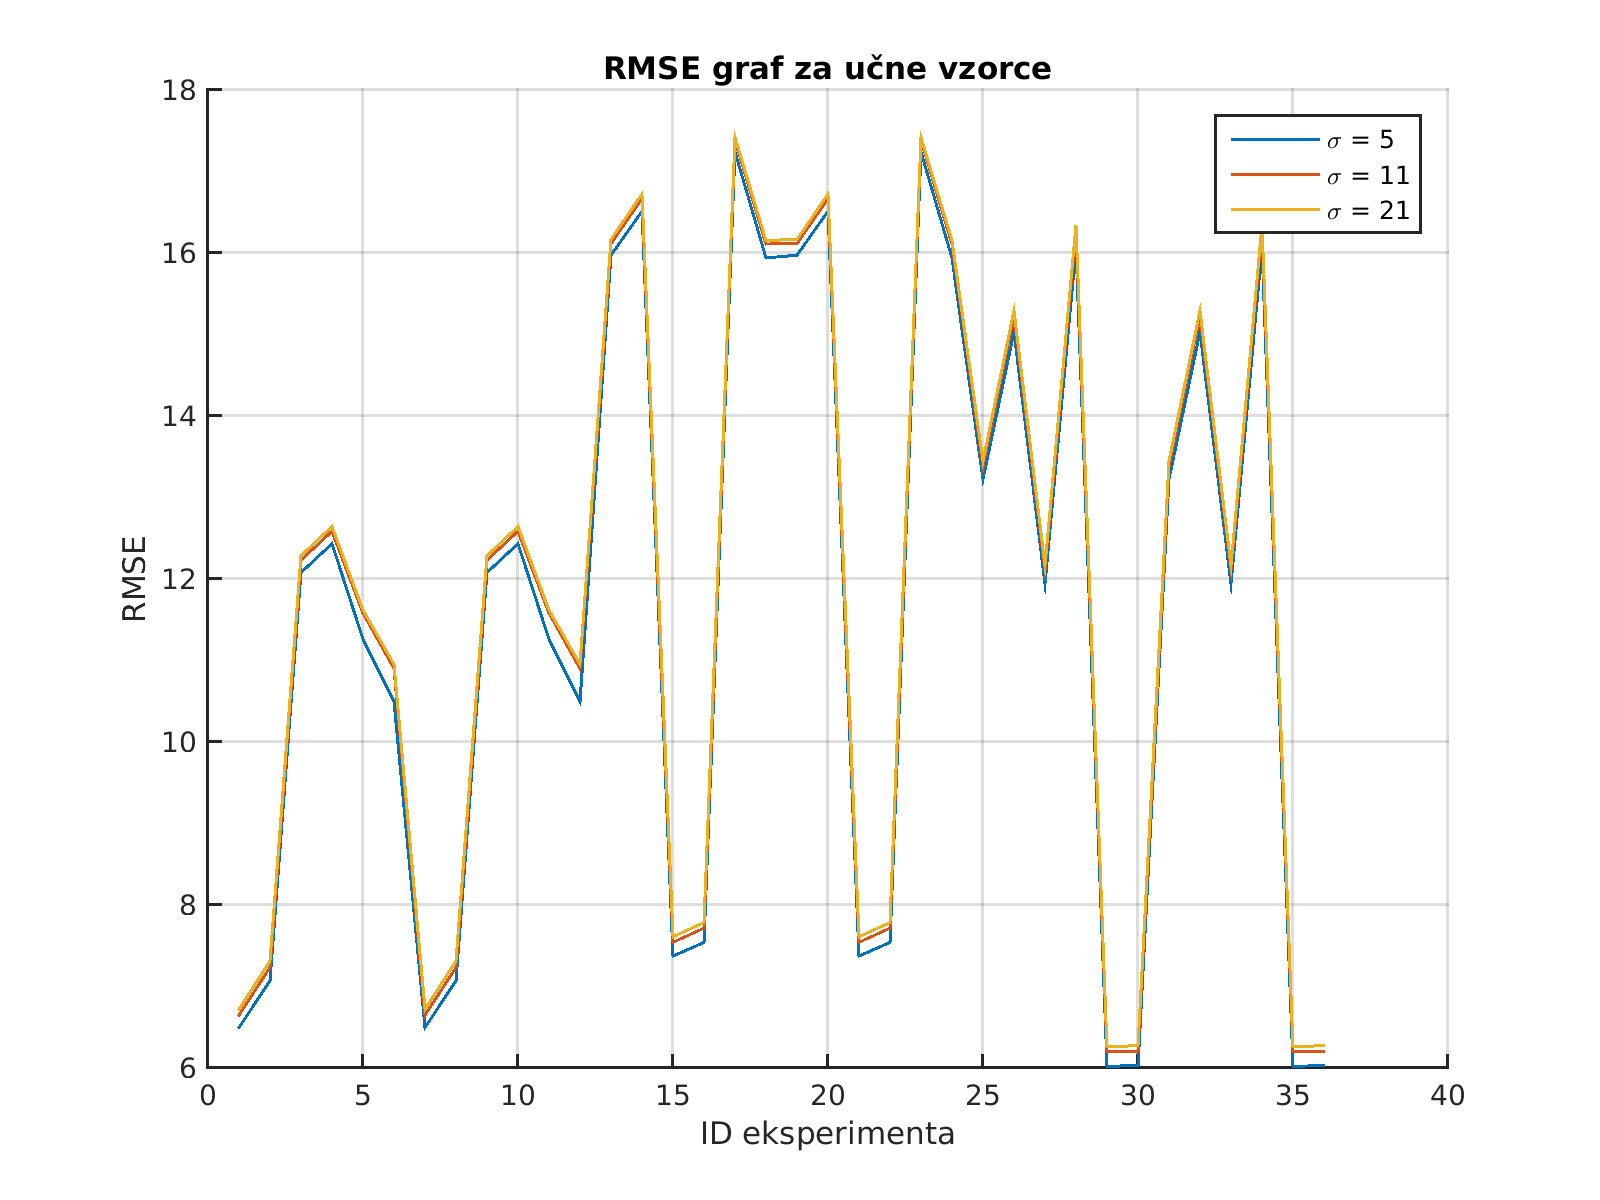
\includegraphics[width=\columnwidth]{./Slike/sigma-rmse5-21.png}
		\caption{Graf RMSE  učnih vzorcev}
		\label{fig:sigma-rmse5-21}
	\end{subfigure}
	~
	\begin{subfigure}[t]{0.45\columnwidth}
		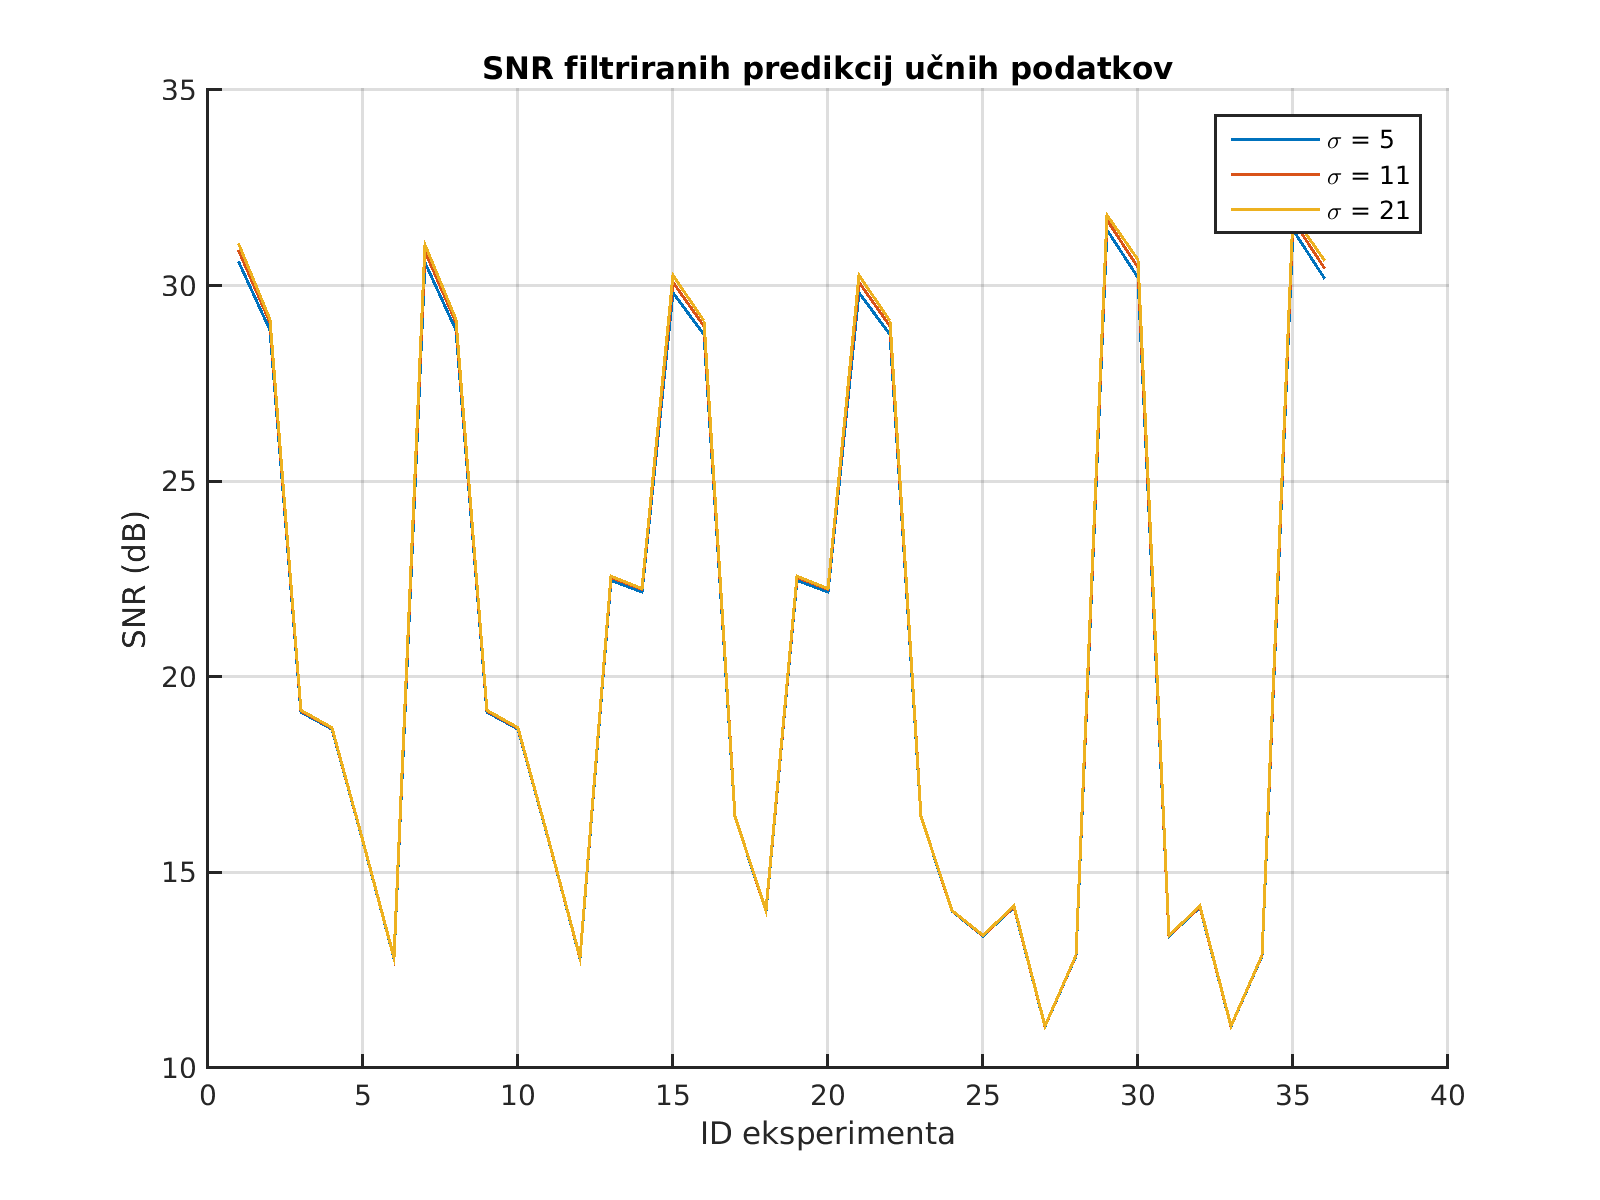
\includegraphics[width=\columnwidth]{./Slike/sigma-snr5-21.png}
		\caption{Graf SNR  učnih vzorcev}
		\label{fig:sigma-snr5-21}
	\end{subfigure}
	\caption{Grafa RMSE in SNR učnih vzorcev za \mbox{$\sigma \in [5,21]$}}
	\label{fig:sigma5-21}
\end{figure}



\begin{figure}[htb]
	\centering
	\begin{subfigure}[t]{0.45\columnwidth}
		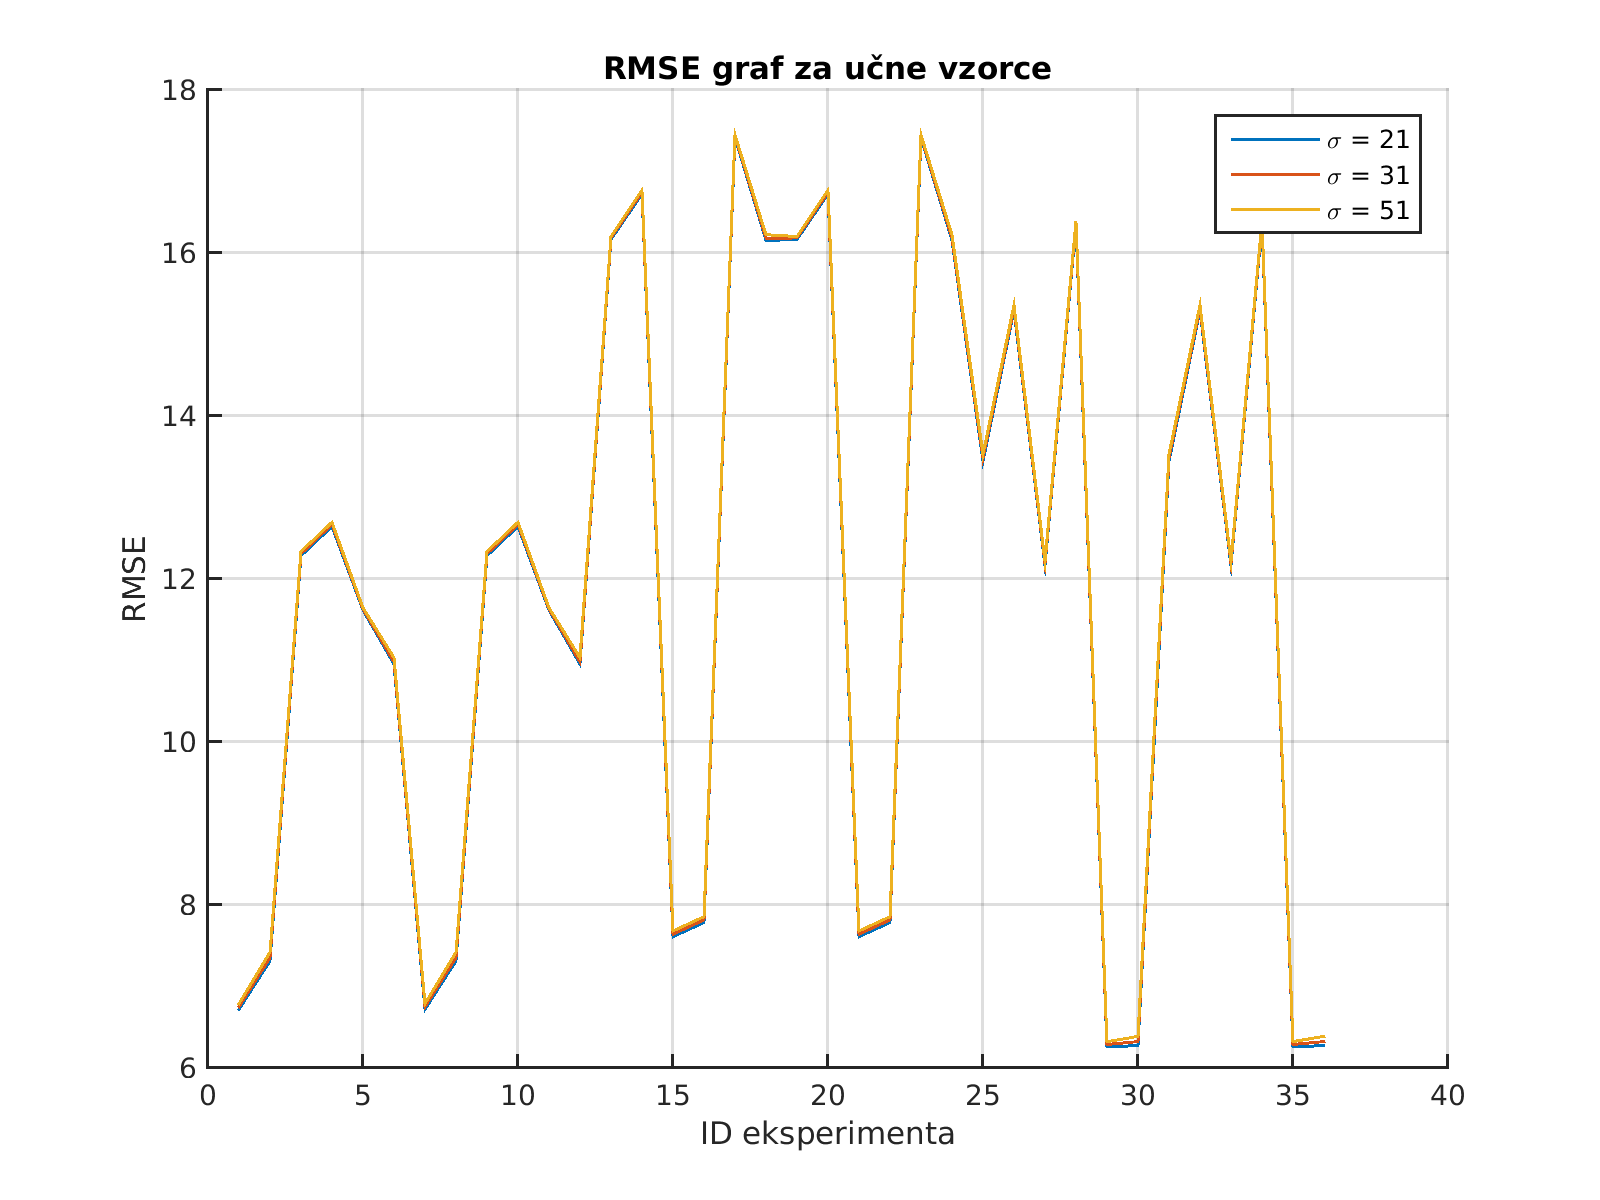
\includegraphics[width=\columnwidth]{./Slike/sigma-rmse21-51.png}
		\caption{Graf RMSE učnih vzorcev}
		\label{fig:sigma-rmse21-51}
	\end{subfigure}
	~
	\begin{subfigure}[t]{0.45\columnwidth}
		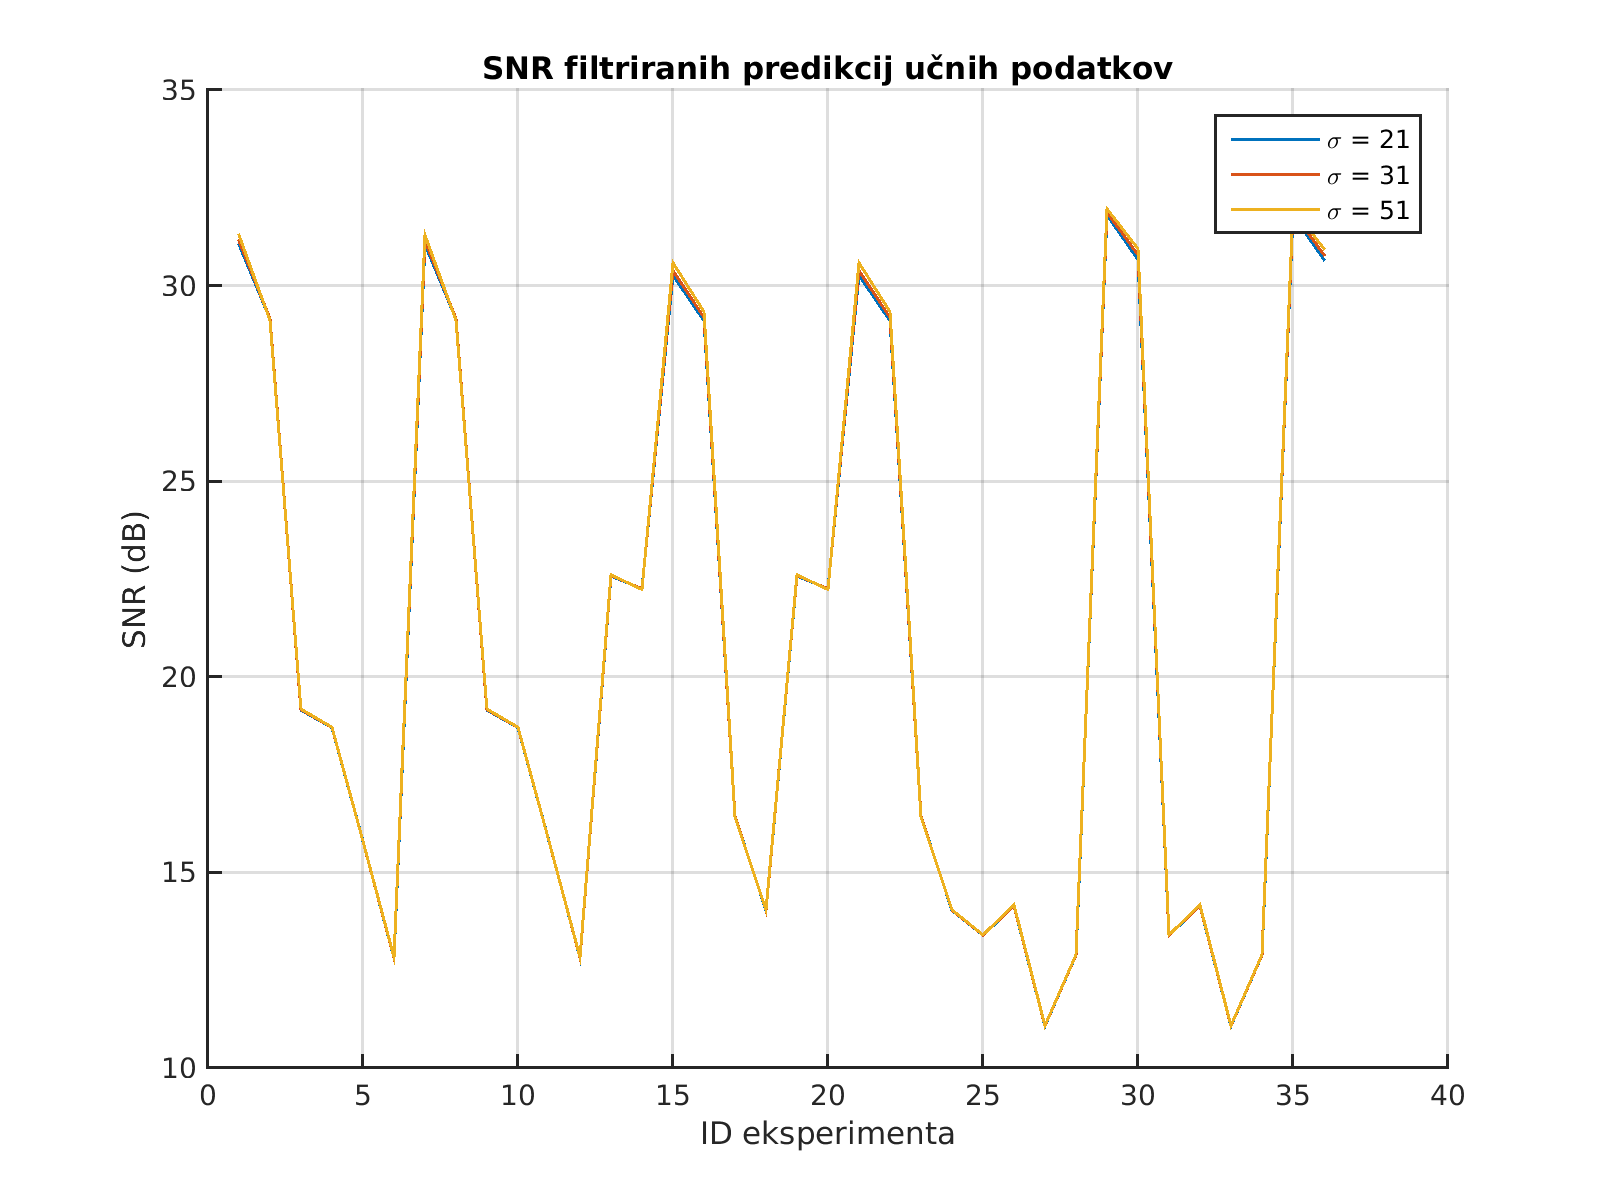
\includegraphics[width=\columnwidth]{./Slike/sigma-snr21-51.png}
		\caption{Graf SNR  učnih vzorcev}
		\label{fig:sigma-snr21-51}
	\end{subfigure}
	\caption{Grafa RMSE in SNR učnih vzorcev za \mbox{$\sigma \in [21,51]$}}
	\label{fig:sigma21-51}
\end{figure}






\subsubsection{Normalizacija HAFA deskriptorja}

\begin{table}[htb]
	\centering
	\begin{tabular}{l S[table-format=1.3] S[table-format=2.3] S[table-format=2.3] S[table-format=2.2]}
		\toprule
		\thead{$\mathbf{Model}$} & \thead{$\mathbf{r}$} & \thead{RAE} & \thead{RRSE} & \thead{nSV [\%]}\\
		\midrule%nSV
		NORMAL & 0.001 & 30.887 & 28.416 & 14.31 \\
		DIAG & -0.151 & 11.217 & 11.380 & 14.31 \\
		\bottomrule
	\end{tabular}
	\caption[]{}
	\label{tab:hafa-norm}
\end{table}

\begin{figure}[htb]
	\centering
	\begin{subfigure}[t]{0.45\columnwidth}
		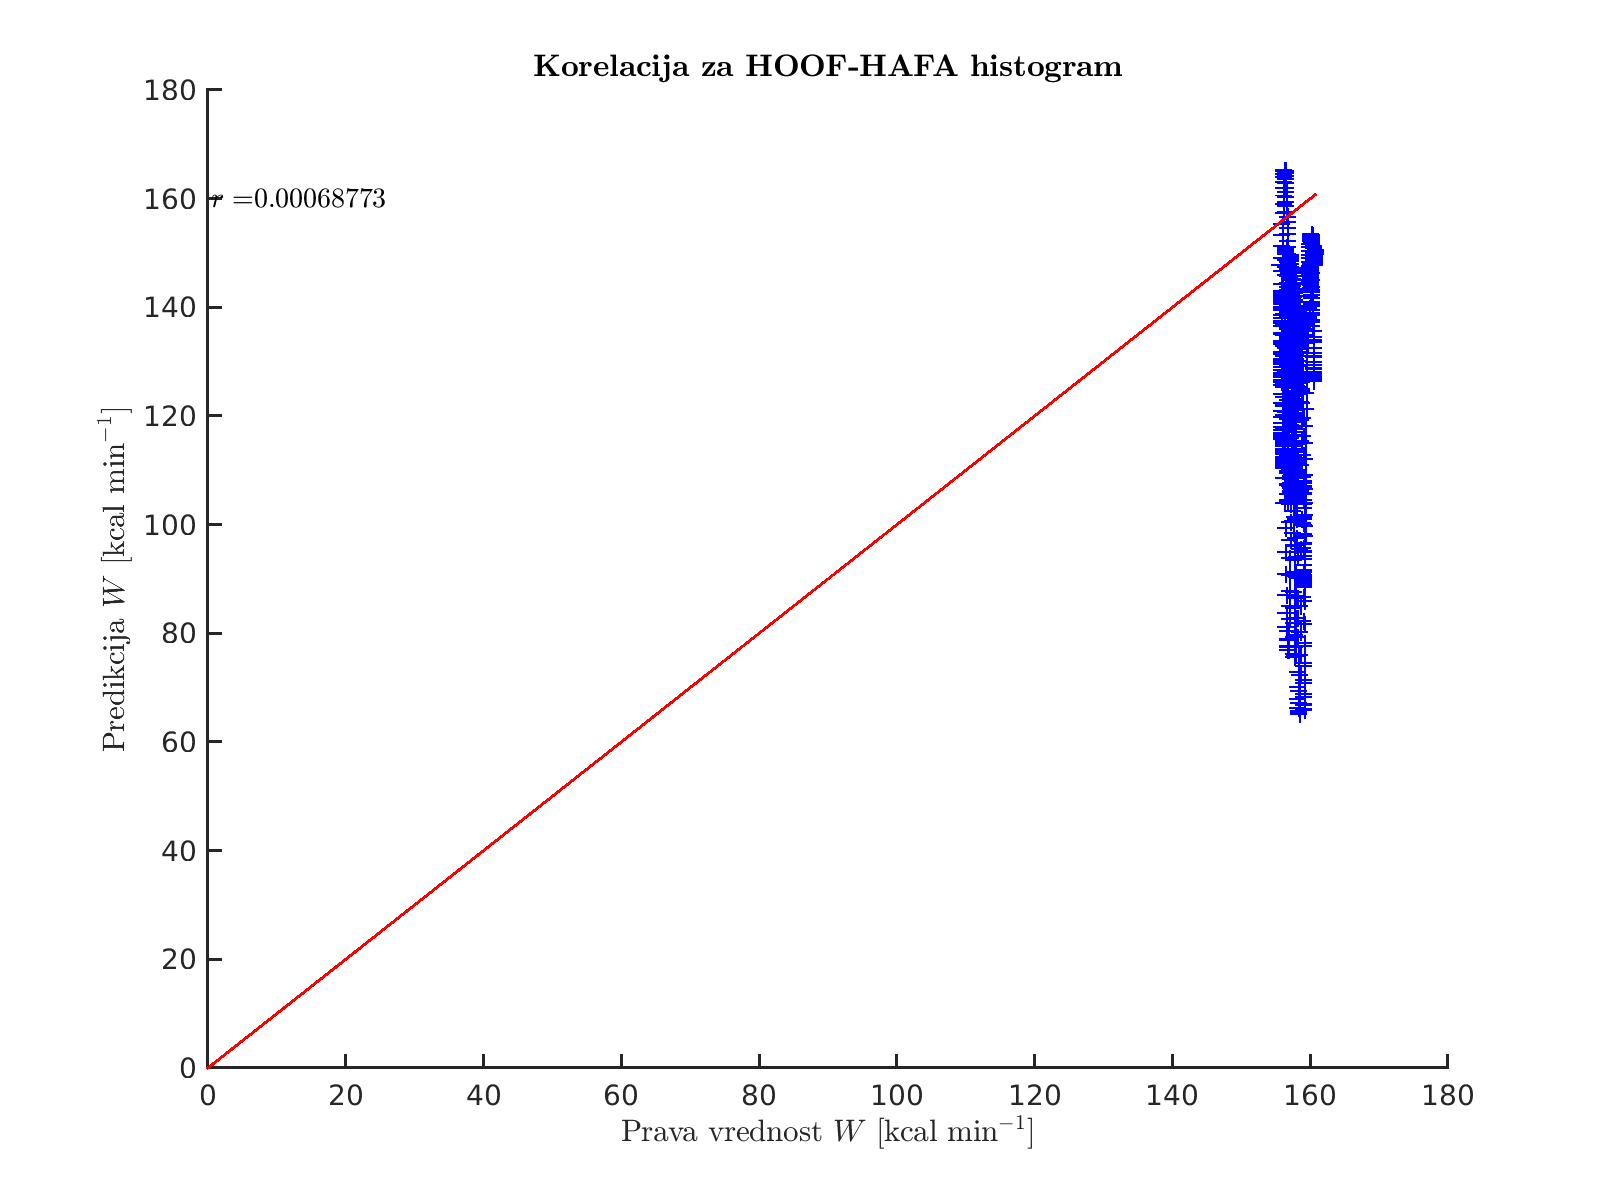
\includegraphics[width=\columnwidth]{./Slike/diag-normal-corr.png}
		\caption{Korelacija.}
		\label{fig:corr-diag-normal}
	\end{subfigure}
	~
	\begin{subfigure}[t]{0.45\columnwidth}
		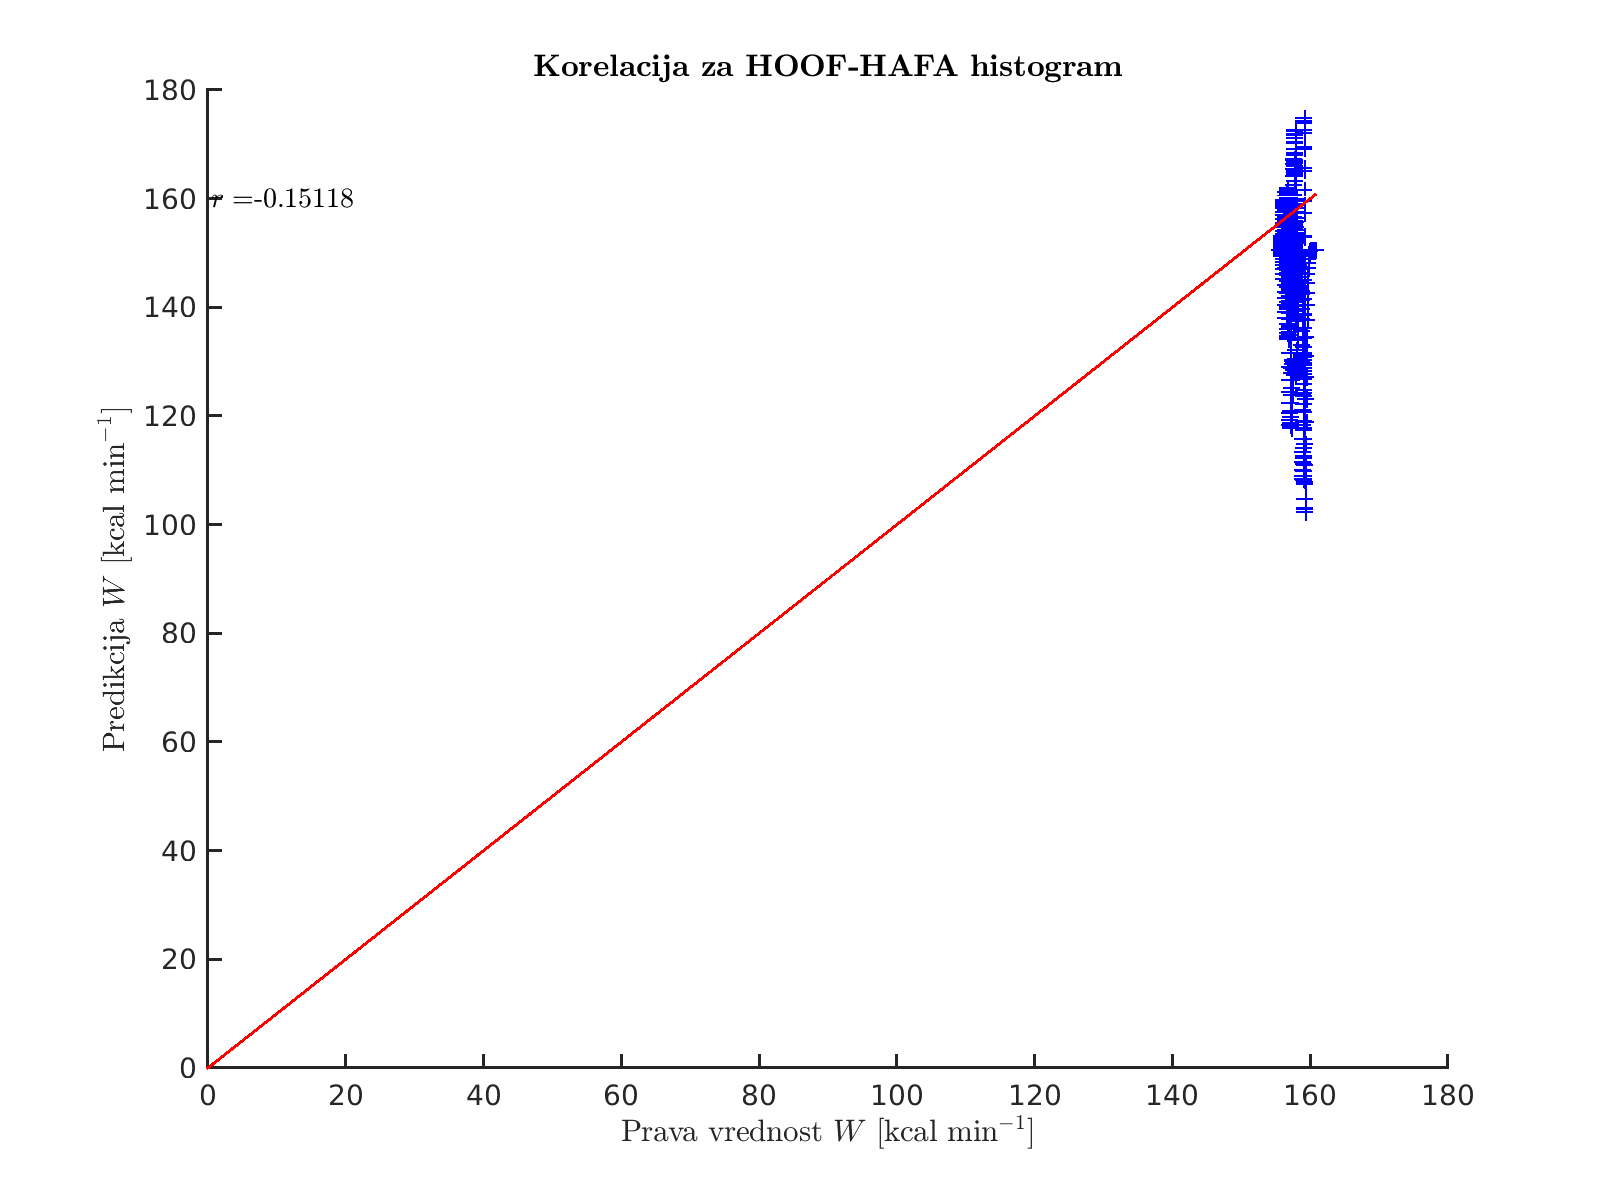
\includegraphics[width=\columnwidth]{./Slike/diag-diag-corr.png}
		\caption{Korelacija.}
		\label{fig:corr-diag-diag}
	\end{subfigure}
	\caption[]{}
	\label{fig:corr-diag}
\end{figure}


\subsection{Laboratorijski eksperiementi}









\subsubsection{Protokol 1}











\subsubsection{Protokol 2}











\subsubsection{Protokol 3}












\subsection{Terenski eksperimenti}











\subsubsection{Protokol 1}














\subsubsection{Protokol 2}









\subsubsection{Protokol 3}










